%\documentclass[a4paper,10pt]{article}
\documentclass[10pt]{scrartcl}
%\usepackage[IL2]{fontenc}
\usepackage[utf8x]{inputenc}
\usepackage[czech]{babel}
\usepackage{listings}  
\usepackage{amsfonts,amsmath,amssymb,graphicx,color}
%\usepackage[total={17cm,27cm}, top=2cm, left=2cm, includefoot]{geometry}
%\usepackage{fancyhdr}
\usepackage{fkssugar}
\usepackage{hyperref}
\usepackage{mhchem}

%\usepackage{caption}

%  Umožňuje rozdělovat obsah na více sloupců
\usepackage{multicol}
\usepackage{booktabs}
\usepackage{pgffor}


% FJFI Types of popi
\renewcommand{\popi}[2]{$\frac{#1}{[\jd{#2}]}$}

\renewcommand{\figurename}{Obr.}
\addto\captionsczech{\renewcommand{\figurename}{Obr.}}
\addto\captionsczech{\renewcommand{\tablename}{Tab.}}
\def\mean#1{\left< #1 \right>}


\newcommand{\MakeFJFIHead}{
\setlength{\parindent}{0cm}
\begin{multicols}{2}
\textsf{\textbf{\FJFISubject \hspace{6.25cm} \FJFIInstitute}\\
\textbf{\large{\FJFITitle}}}

\begin{tabular}{rlrl}
	 \textsf{Jméno:} & \textbf{\textsf\FJFIAuthor}    &      \textsf{Kolega:} & \textsf{\FJFICoauthor} \\[1.5pt]
	  \textsf{Kruh:} & \textbf{\textsf\FJFIGroup}     & \textsf{Číslo skup.:} & \textsf{\FJFICircle}   \\[1.5pt]
	\textsf{Měřeno:} & \textbf{\textsf{\FJFILabdate}} &  \textsf{Zpracování}: & \textsf{\FJFIWorktime}
\end{tabular}

\begin{flushright}


\includegraphics[scale=0.2]{../img/fjfi.pdf}
%\hspace{0.4cm}
%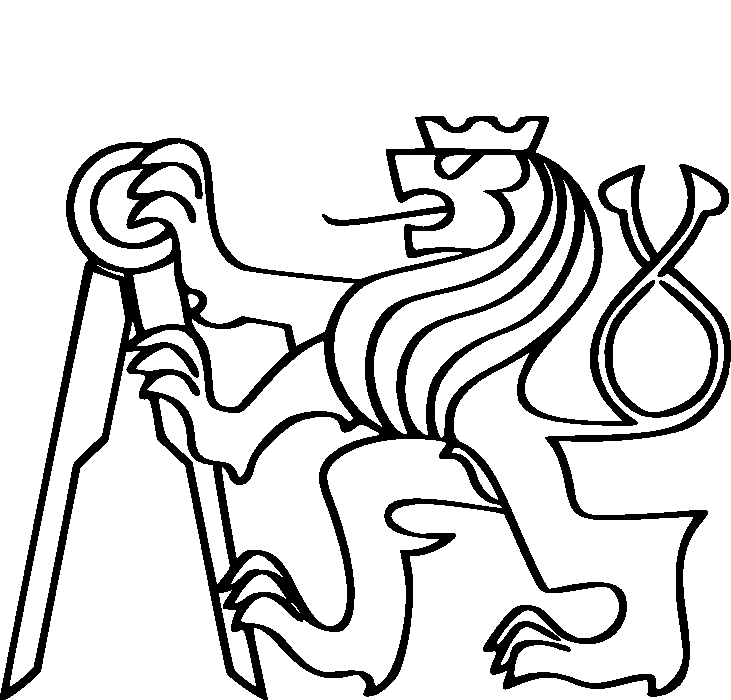
\includegraphics[scale=0.2]{../img/cvut.pdf}


\textsf{Klasifikace:} \hspace{3.2cm} 

\end{flushright}
\end{multicols}

\hrule
}




%  Nastaví autora, název, datum, skupinu měření apod. 
\newcommand{\FJFIInstitute}{FJFI~ČVUT~v~Praze}
%\newcommand{\Subject}{Základy fyzikálních měření}
\newcommand{\FJFISubject}{Fyzikální praktikum I}  %odkomentujte dle potřeby

%  Máte-li více spoluměřících než jednoho, vložte jen jejich příjmení
\newcommand{\FJFIAuthor}{Michal Červeňák}
\newcommand{\FJFICoauthor}{} 
\newcommand{\FJFIGroup}{Útorok} %den, kdy chodíte na praktika, nikoli obor
\newcommand{\FJFICircle}{1} %číslo skupiny v rámci praktika, nikoli kruh

%  Tato část bude v každém protokolu jiná, nezapomeňte upravit!
\newcommand{\FJFITitle}{4. Cavendishův experiment}
\newcommand{\FJFILabdate}{9.10.2017} %datum měření, nikoli datum odevzdání
\newcommand{\FJFIWorktime}{3 h} %jak dlouho vám trvalo vypracování protokolu


\begin{document}

\MakeFJFIHead{}

\section{Pracovní úkol}
\begin{enumerate}
\item DU: Zopakujte si výpočet chyb nepřímého měřen´ı, vysvětlete rozdíl mezi lineárním 
a kvadratickým zákonem hromadění chyb a jejich použití.
\item DU: Odvoďťe vztah pro výpočet relativní chyby měření $G$ a zamyslete se, jak
vypadá chyba periody kmitu $T$ a chyba rozdílu vzdáleností rovnovážných poloh $S$.
\item DU: V přípravě odvoďťe vztah pro výpočet relativní chyby měření $G$ a zamyslete
se, jak vypadá chyba periody kmitu $T$ a chyba rozdílu vzdáleností
rovnovážných poloh $S$.
\item Ve spolupráci s asistentem zkontrolujte, zda je torzní kyvadlo horizontálně vyrovnané.
($"20 min"$)
\item Pomocí torzního kyvadla změřte gravitační konstantu. Do protokolu přiložte graf naměřených
dat včetně odchylek a nafitované funkce. Diskutujte, zda bylo kyvadlo rotačně vyrovnané.


\end{enumerate}

\section{Postup merania}

\begin{enumerate}
\item Najskôr bola aparatúra horizontálne vyrovnaná a dôkladne skontrolované jej vyváženie.
\item Následne boli na držiaky osadené gule, a prítlačné  na doraz do prvej polohy.
\item Aparatúra sa odaretovala a nechala sa kmitať dokedy sa pri kmitoch neprestali guličky dotýkať od stien.
\item Podobu $\sim$ 3 kmitov sa zaznamenávala zmena výchylky laserového paprsku na čase, v našom prípade každých $"20 s"$.
\item Gule boli otočné do druhej polohy a opakovalo sa meranie pre 3 kmity.
\item Pomocou metru bola odmeraná vzdialenosť kyvadla od steny, na ktorú sa odčítavala vzdialenosť. 
\end{enumerate}

\section{Pomôcky}
Torzné kyvadlo, zemniacé káble, radiátor, laser, ochranné okuliare, podstavec pod laser,
stopky, meter provázek.

\section{Teória}
Newtonov gravitačný zákon hovorí, že gravitačná sila $F$ medzi dvoma telesami je priamo úmerná ich hmotnostiam $m_1$ a $m_2$ a nepriamo štvorci vzdialenosti $r$, teda
\eq{
F = G\frac{m_1 m_2}{r^2}\,,
}
kde $G$ je gravitačná konštanta, ktorá udáva veľkosť interakcie.

Zo vzorcov pre torzné kyvadlo a gravitačného zákona sa dá odvodiť vzťah
\eq{
G = \frac{\pi^2 b^2}{m_2 d} \frac{d^2 + \frac{2}{5}r^2}{\(1-\frac{b^3}{b^2+4d^2}^{3/2}\)} \frac{S}{T^2 L}\,, \\ \lbl{R_2}
} pričom 
\eq[m]{
r = "9,55 mm"\,, \\
d = "50,7 mm"\,, \\
b = "45 mm"\,, \\
S = S^2 - S^1 \,, \\
m_2 = "1,24 kg"\,,
}
kde $m_2$ je hmotnosť, každej z olovených gúľ, 
$S$ je rozdeľ nulových polôh kmitov v jednotlivých polohách $S^i$,
$b$ je vzdialenosť stredov malej a veľkej gule,
$d$ je vzdialenosť stredu malej gule od stredu osi otáčania torzného kyvadla,
a $r$ je polomer malej gule.
 
Vzťah pre tlmené harmonické kmity\eq{
f(t) = A\exp\(-\delta t\) \sin\( \frac{2*\pi}{T}t + \sigma\) + S^{1\(2\)} \lbl{R_1}\,.
}


\subsubsection{Spracovanie chýb merania}

Označme $\mean{t}$ aritmetický priemer nameraných hodnôt $t_i$, a $\Delta t$ hodnotu $\mean{t}-t$, pričom 
\eq{
\mean{t} = \frac{1}{n}\sum_{i=1}^n t_i \,, \lbl{SCH_1}
}  
a chybu aritmetického priemeru 
\eq{
  \sigma_0=\sqrt{\frac{\sum_{i=1}^n \(t_i - \mean{t}\)^2}{n\(n-1\)}}\,, \lbl{SCH_2}
}
pričom $n$ je počet meraní.

Majme veličina  $ u = f(x,y,z,\ldots)$, potom podľa zákou šírenia chýb platí
\eq{
\sigma_u = \sqrt{\(\pder{f}{x}\)^2_0 \sigma_x^2 +\(\pder{f}{y}\)^2_0 \sigma_y^2 + \(\pder{f}{z}\)^2_0 \sigma_z^2 + \ldots}\,, \lbl{SCH_3}
}
kde $\sigma_i$ je stredná chyba veličiny $i$ v bode $\(x_0,y_0,z_0\)$.




Vzorec \ref{R_2} sa dá pre naše účely prepísať ako \eq{
G = \const \frac{S}{T^2 L}\,,
} z čoho môže odvodiť pre chybu merania
\eq{
\frac{\Delta G}{\mid G\mid } = \frac{\Delta S}{\mid S\mid } +\frac{2\Delta T}{\mid T\mid } +\frac{\Delta L}{\mid L\mid } \,. \lbl{R_3}
}




\section{Výsledky merania}

Namerané dáta sú vynesené do grafu Obr. \ref{G_1}. 
Následne pre obe polohy gulí boli dáta preložené závislosťou \eqref{R_1}, a z nej zistené hodnoty \eq[m]{
S^1 = "\(115.6\pm 0.3\) cm" \,,\\
S^2 = "\(125.6\pm 0.1\) cm" \,,\\
T = "\(493.6\pm 0.4\) s" \,.\\
}
Preloženie je v Obr. \ref{G_2} a Obr. \ref{G_3}, a v Obr. \ref{G_4} sú vykreslené spolu s dátami a fitmi aj hodnoty $S^1$ a $S^2$.

Metrom bola odmeraná hodnota $L = "\(598\pm5\) cm"$, nepresnosť merania bola odhadnutá na $"5 cm"$ hlavne z dôvodu merania popri stene a postupného merania.
Nepresnosť určovania času bola stanovená na $"5 s"$.

Po dosadení do vzorca \eqref{R_2} a \eqref{R_3}, bola dopočítaná hodnota $G = "\(5.71\pm0.95\)\cdot10^{-11} m^3 \cdot kg^{-1}\cdot s^{-2}"$.

\begin{figure}
% GNUPLOT: LaTeX picture
\setlength{\unitlength}{0.240900pt}
\ifx\plotpoint\undefined\newsavebox{\plotpoint}\fi
\begin{picture}(1500,900)(0,0)
\sbox{\plotpoint}{\rule[-0.200pt]{0.400pt}{0.400pt}}%
\put(191.0,131.0){\rule[-0.200pt]{4.818pt}{0.400pt}}
\put(171,131){\makebox(0,0)[r]{ 1.15}}
\put(1419.0,131.0){\rule[-0.200pt]{4.818pt}{0.400pt}}
\put(191.0,252.0){\rule[-0.200pt]{4.818pt}{0.400pt}}
\put(171,252){\makebox(0,0)[r]{ 1.2}}
\put(1419.0,252.0){\rule[-0.200pt]{4.818pt}{0.400pt}}
\put(191.0,374.0){\rule[-0.200pt]{4.818pt}{0.400pt}}
\put(171,374){\makebox(0,0)[r]{ 1.25}}
\put(1419.0,374.0){\rule[-0.200pt]{4.818pt}{0.400pt}}
\put(191.0,495.0){\rule[-0.200pt]{4.818pt}{0.400pt}}
\put(171,495){\makebox(0,0)[r]{ 1.3}}
\put(1419.0,495.0){\rule[-0.200pt]{4.818pt}{0.400pt}}
\put(191.0,616.0){\rule[-0.200pt]{4.818pt}{0.400pt}}
\put(171,616){\makebox(0,0)[r]{ 1.35}}
\put(1419.0,616.0){\rule[-0.200pt]{4.818pt}{0.400pt}}
\put(191.0,738.0){\rule[-0.200pt]{4.818pt}{0.400pt}}
\put(171,738){\makebox(0,0)[r]{ 1.4}}
\put(1419.0,738.0){\rule[-0.200pt]{4.818pt}{0.400pt}}
\put(191.0,859.0){\rule[-0.200pt]{4.818pt}{0.400pt}}
\put(171,859){\makebox(0,0)[r]{ 1.45}}
\put(1419.0,859.0){\rule[-0.200pt]{4.818pt}{0.400pt}}
\put(191.0,131.0){\rule[-0.200pt]{0.400pt}{4.818pt}}
\put(191,90){\makebox(0,0){ 0}}
\put(191.0,839.0){\rule[-0.200pt]{0.400pt}{4.818pt}}
\put(316.0,131.0){\rule[-0.200pt]{0.400pt}{4.818pt}}
\put(316,90){\makebox(0,0){ 0.05}}
\put(316.0,839.0){\rule[-0.200pt]{0.400pt}{4.818pt}}
\put(441.0,131.0){\rule[-0.200pt]{0.400pt}{4.818pt}}
\put(441,90){\makebox(0,0){ 0.1}}
\put(441.0,839.0){\rule[-0.200pt]{0.400pt}{4.818pt}}
\put(565.0,131.0){\rule[-0.200pt]{0.400pt}{4.818pt}}
\put(565,90){\makebox(0,0){ 0.15}}
\put(565.0,839.0){\rule[-0.200pt]{0.400pt}{4.818pt}}
\put(690.0,131.0){\rule[-0.200pt]{0.400pt}{4.818pt}}
\put(690,90){\makebox(0,0){ 0.2}}
\put(690.0,839.0){\rule[-0.200pt]{0.400pt}{4.818pt}}
\put(815.0,131.0){\rule[-0.200pt]{0.400pt}{4.818pt}}
\put(815,90){\makebox(0,0){ 0.25}}
\put(815.0,839.0){\rule[-0.200pt]{0.400pt}{4.818pt}}
\put(940.0,131.0){\rule[-0.200pt]{0.400pt}{4.818pt}}
\put(940,90){\makebox(0,0){ 0.3}}
\put(940.0,839.0){\rule[-0.200pt]{0.400pt}{4.818pt}}
\put(1065.0,131.0){\rule[-0.200pt]{0.400pt}{4.818pt}}
\put(1065,90){\makebox(0,0){ 0.35}}
\put(1065.0,839.0){\rule[-0.200pt]{0.400pt}{4.818pt}}
\put(1189.0,131.0){\rule[-0.200pt]{0.400pt}{4.818pt}}
\put(1189,90){\makebox(0,0){ 0.4}}
\put(1189.0,839.0){\rule[-0.200pt]{0.400pt}{4.818pt}}
\put(1314.0,131.0){\rule[-0.200pt]{0.400pt}{4.818pt}}
\put(1314,90){\makebox(0,0){ 0.45}}
\put(1314.0,839.0){\rule[-0.200pt]{0.400pt}{4.818pt}}
\put(1439.0,131.0){\rule[-0.200pt]{0.400pt}{4.818pt}}
\put(1439,90){\makebox(0,0){ 0.5}}
\put(1439.0,839.0){\rule[-0.200pt]{0.400pt}{4.818pt}}
\put(191.0,131.0){\rule[-0.200pt]{0.400pt}{175.375pt}}
\put(191.0,131.0){\rule[-0.200pt]{300.643pt}{0.400pt}}
\put(1439.0,131.0){\rule[-0.200pt]{0.400pt}{175.375pt}}
\put(191.0,859.0){\rule[-0.200pt]{300.643pt}{0.400pt}}
\put(30,495){\makebox(0,0){\popi{\kappa}{-}}}
\put(815,29){\makebox(0,0){\popi{t}{s}}}
\put(1279,819){\makebox(0,0)[r]{linenárny fit pre $t<"200 ms"$}}
\put(1299.0,819.0){\rule[-0.200pt]{24.090pt}{0.400pt}}
\put(308,603){\usebox{\plotpoint}}
\multiput(308.00,601.94)(1.505,-0.468){5}{\rule{1.200pt}{0.113pt}}
\multiput(308.00,602.17)(8.509,-4.000){2}{\rule{0.600pt}{0.400pt}}
\multiput(319.00,597.95)(2.248,-0.447){3}{\rule{1.567pt}{0.108pt}}
\multiput(319.00,598.17)(7.748,-3.000){2}{\rule{0.783pt}{0.400pt}}
\multiput(330.00,594.94)(1.505,-0.468){5}{\rule{1.200pt}{0.113pt}}
\multiput(330.00,595.17)(8.509,-4.000){2}{\rule{0.600pt}{0.400pt}}
\multiput(341.00,590.95)(2.248,-0.447){3}{\rule{1.567pt}{0.108pt}}
\multiput(341.00,591.17)(7.748,-3.000){2}{\rule{0.783pt}{0.400pt}}
\multiput(352.00,587.94)(1.505,-0.468){5}{\rule{1.200pt}{0.113pt}}
\multiput(352.00,588.17)(8.509,-4.000){2}{\rule{0.600pt}{0.400pt}}
\multiput(363.00,583.94)(1.505,-0.468){5}{\rule{1.200pt}{0.113pt}}
\multiput(363.00,584.17)(8.509,-4.000){2}{\rule{0.600pt}{0.400pt}}
\multiput(374.00,579.95)(2.248,-0.447){3}{\rule{1.567pt}{0.108pt}}
\multiput(374.00,580.17)(7.748,-3.000){2}{\rule{0.783pt}{0.400pt}}
\multiput(385.00,576.94)(1.505,-0.468){5}{\rule{1.200pt}{0.113pt}}
\multiput(385.00,577.17)(8.509,-4.000){2}{\rule{0.600pt}{0.400pt}}
\multiput(396.00,572.94)(1.505,-0.468){5}{\rule{1.200pt}{0.113pt}}
\multiput(396.00,573.17)(8.509,-4.000){2}{\rule{0.600pt}{0.400pt}}
\multiput(407.00,568.95)(2.248,-0.447){3}{\rule{1.567pt}{0.108pt}}
\multiput(407.00,569.17)(7.748,-3.000){2}{\rule{0.783pt}{0.400pt}}
\multiput(418.00,565.94)(1.505,-0.468){5}{\rule{1.200pt}{0.113pt}}
\multiput(418.00,566.17)(8.509,-4.000){2}{\rule{0.600pt}{0.400pt}}
\multiput(429.00,561.94)(1.505,-0.468){5}{\rule{1.200pt}{0.113pt}}
\multiput(429.00,562.17)(8.509,-4.000){2}{\rule{0.600pt}{0.400pt}}
\multiput(440.00,557.95)(2.248,-0.447){3}{\rule{1.567pt}{0.108pt}}
\multiput(440.00,558.17)(7.748,-3.000){2}{\rule{0.783pt}{0.400pt}}
\multiput(451.00,554.94)(1.505,-0.468){5}{\rule{1.200pt}{0.113pt}}
\multiput(451.00,555.17)(8.509,-4.000){2}{\rule{0.600pt}{0.400pt}}
\multiput(462.00,550.94)(1.505,-0.468){5}{\rule{1.200pt}{0.113pt}}
\multiput(462.00,551.17)(8.509,-4.000){2}{\rule{0.600pt}{0.400pt}}
\multiput(473.00,546.95)(2.248,-0.447){3}{\rule{1.567pt}{0.108pt}}
\multiput(473.00,547.17)(7.748,-3.000){2}{\rule{0.783pt}{0.400pt}}
\multiput(484.00,543.94)(1.505,-0.468){5}{\rule{1.200pt}{0.113pt}}
\multiput(484.00,544.17)(8.509,-4.000){2}{\rule{0.600pt}{0.400pt}}
\multiput(495.00,539.94)(1.505,-0.468){5}{\rule{1.200pt}{0.113pt}}
\multiput(495.00,540.17)(8.509,-4.000){2}{\rule{0.600pt}{0.400pt}}
\multiput(506.00,535.95)(2.248,-0.447){3}{\rule{1.567pt}{0.108pt}}
\multiput(506.00,536.17)(7.748,-3.000){2}{\rule{0.783pt}{0.400pt}}
\multiput(517.00,532.94)(1.505,-0.468){5}{\rule{1.200pt}{0.113pt}}
\multiput(517.00,533.17)(8.509,-4.000){2}{\rule{0.600pt}{0.400pt}}
\multiput(528.00,528.94)(1.505,-0.468){5}{\rule{1.200pt}{0.113pt}}
\multiput(528.00,529.17)(8.509,-4.000){2}{\rule{0.600pt}{0.400pt}}
\multiput(539.00,524.95)(2.248,-0.447){3}{\rule{1.567pt}{0.108pt}}
\multiput(539.00,525.17)(7.748,-3.000){2}{\rule{0.783pt}{0.400pt}}
\multiput(550.00,521.94)(1.505,-0.468){5}{\rule{1.200pt}{0.113pt}}
\multiput(550.00,522.17)(8.509,-4.000){2}{\rule{0.600pt}{0.400pt}}
\multiput(561.00,517.95)(2.248,-0.447){3}{\rule{1.567pt}{0.108pt}}
\multiput(561.00,518.17)(7.748,-3.000){2}{\rule{0.783pt}{0.400pt}}
\multiput(572.00,514.94)(1.358,-0.468){5}{\rule{1.100pt}{0.113pt}}
\multiput(572.00,515.17)(7.717,-4.000){2}{\rule{0.550pt}{0.400pt}}
\multiput(582.00,510.94)(1.505,-0.468){5}{\rule{1.200pt}{0.113pt}}
\multiput(582.00,511.17)(8.509,-4.000){2}{\rule{0.600pt}{0.400pt}}
\multiput(593.00,506.95)(2.248,-0.447){3}{\rule{1.567pt}{0.108pt}}
\multiput(593.00,507.17)(7.748,-3.000){2}{\rule{0.783pt}{0.400pt}}
\multiput(604.00,503.94)(1.505,-0.468){5}{\rule{1.200pt}{0.113pt}}
\multiput(604.00,504.17)(8.509,-4.000){2}{\rule{0.600pt}{0.400pt}}
\multiput(615.00,499.94)(1.505,-0.468){5}{\rule{1.200pt}{0.113pt}}
\multiput(615.00,500.17)(8.509,-4.000){2}{\rule{0.600pt}{0.400pt}}
\multiput(626.00,495.95)(2.248,-0.447){3}{\rule{1.567pt}{0.108pt}}
\multiput(626.00,496.17)(7.748,-3.000){2}{\rule{0.783pt}{0.400pt}}
\multiput(637.00,492.94)(1.505,-0.468){5}{\rule{1.200pt}{0.113pt}}
\multiput(637.00,493.17)(8.509,-4.000){2}{\rule{0.600pt}{0.400pt}}
\multiput(648.00,488.94)(1.505,-0.468){5}{\rule{1.200pt}{0.113pt}}
\multiput(648.00,489.17)(8.509,-4.000){2}{\rule{0.600pt}{0.400pt}}
\multiput(659.00,484.95)(2.248,-0.447){3}{\rule{1.567pt}{0.108pt}}
\multiput(659.00,485.17)(7.748,-3.000){2}{\rule{0.783pt}{0.400pt}}
\multiput(670.00,481.94)(1.505,-0.468){5}{\rule{1.200pt}{0.113pt}}
\multiput(670.00,482.17)(8.509,-4.000){2}{\rule{0.600pt}{0.400pt}}
\multiput(681.00,477.94)(1.505,-0.468){5}{\rule{1.200pt}{0.113pt}}
\multiput(681.00,478.17)(8.509,-4.000){2}{\rule{0.600pt}{0.400pt}}
\multiput(692.00,473.95)(2.248,-0.447){3}{\rule{1.567pt}{0.108pt}}
\multiput(692.00,474.17)(7.748,-3.000){2}{\rule{0.783pt}{0.400pt}}
\multiput(703.00,470.94)(1.505,-0.468){5}{\rule{1.200pt}{0.113pt}}
\multiput(703.00,471.17)(8.509,-4.000){2}{\rule{0.600pt}{0.400pt}}
\multiput(714.00,466.94)(1.505,-0.468){5}{\rule{1.200pt}{0.113pt}}
\multiput(714.00,467.17)(8.509,-4.000){2}{\rule{0.600pt}{0.400pt}}
\multiput(725.00,462.95)(2.248,-0.447){3}{\rule{1.567pt}{0.108pt}}
\multiput(725.00,463.17)(7.748,-3.000){2}{\rule{0.783pt}{0.400pt}}
\multiput(736.00,459.94)(1.505,-0.468){5}{\rule{1.200pt}{0.113pt}}
\multiput(736.00,460.17)(8.509,-4.000){2}{\rule{0.600pt}{0.400pt}}
\multiput(747.00,455.95)(2.248,-0.447){3}{\rule{1.567pt}{0.108pt}}
\multiput(747.00,456.17)(7.748,-3.000){2}{\rule{0.783pt}{0.400pt}}
\multiput(758.00,452.94)(1.505,-0.468){5}{\rule{1.200pt}{0.113pt}}
\multiput(758.00,453.17)(8.509,-4.000){2}{\rule{0.600pt}{0.400pt}}
\multiput(769.00,448.94)(1.505,-0.468){5}{\rule{1.200pt}{0.113pt}}
\multiput(769.00,449.17)(8.509,-4.000){2}{\rule{0.600pt}{0.400pt}}
\multiput(780.00,444.95)(2.248,-0.447){3}{\rule{1.567pt}{0.108pt}}
\multiput(780.00,445.17)(7.748,-3.000){2}{\rule{0.783pt}{0.400pt}}
\multiput(791.00,441.94)(1.505,-0.468){5}{\rule{1.200pt}{0.113pt}}
\multiput(791.00,442.17)(8.509,-4.000){2}{\rule{0.600pt}{0.400pt}}
\multiput(802.00,437.94)(1.505,-0.468){5}{\rule{1.200pt}{0.113pt}}
\multiput(802.00,438.17)(8.509,-4.000){2}{\rule{0.600pt}{0.400pt}}
\multiput(813.00,433.95)(2.248,-0.447){3}{\rule{1.567pt}{0.108pt}}
\multiput(813.00,434.17)(7.748,-3.000){2}{\rule{0.783pt}{0.400pt}}
\multiput(824.00,430.94)(1.505,-0.468){5}{\rule{1.200pt}{0.113pt}}
\multiput(824.00,431.17)(8.509,-4.000){2}{\rule{0.600pt}{0.400pt}}
\multiput(835.00,426.94)(1.505,-0.468){5}{\rule{1.200pt}{0.113pt}}
\multiput(835.00,427.17)(8.509,-4.000){2}{\rule{0.600pt}{0.400pt}}
\multiput(846.00,422.95)(2.248,-0.447){3}{\rule{1.567pt}{0.108pt}}
\multiput(846.00,423.17)(7.748,-3.000){2}{\rule{0.783pt}{0.400pt}}
\multiput(857.00,419.94)(1.505,-0.468){5}{\rule{1.200pt}{0.113pt}}
\multiput(857.00,420.17)(8.509,-4.000){2}{\rule{0.600pt}{0.400pt}}
\multiput(868.00,415.94)(1.505,-0.468){5}{\rule{1.200pt}{0.113pt}}
\multiput(868.00,416.17)(8.509,-4.000){2}{\rule{0.600pt}{0.400pt}}
\multiput(879.00,411.95)(2.248,-0.447){3}{\rule{1.567pt}{0.108pt}}
\multiput(879.00,412.17)(7.748,-3.000){2}{\rule{0.783pt}{0.400pt}}
\multiput(890.00,408.94)(1.505,-0.468){5}{\rule{1.200pt}{0.113pt}}
\multiput(890.00,409.17)(8.509,-4.000){2}{\rule{0.600pt}{0.400pt}}
\multiput(901.00,404.94)(1.505,-0.468){5}{\rule{1.200pt}{0.113pt}}
\multiput(901.00,405.17)(8.509,-4.000){2}{\rule{0.600pt}{0.400pt}}
\multiput(912.00,400.95)(2.025,-0.447){3}{\rule{1.433pt}{0.108pt}}
\multiput(912.00,401.17)(7.025,-3.000){2}{\rule{0.717pt}{0.400pt}}
\multiput(922.00,397.94)(1.505,-0.468){5}{\rule{1.200pt}{0.113pt}}
\multiput(922.00,398.17)(8.509,-4.000){2}{\rule{0.600pt}{0.400pt}}
\multiput(933.00,393.95)(2.248,-0.447){3}{\rule{1.567pt}{0.108pt}}
\multiput(933.00,394.17)(7.748,-3.000){2}{\rule{0.783pt}{0.400pt}}
\multiput(944.00,390.94)(1.505,-0.468){5}{\rule{1.200pt}{0.113pt}}
\multiput(944.00,391.17)(8.509,-4.000){2}{\rule{0.600pt}{0.400pt}}
\multiput(955.00,386.94)(1.505,-0.468){5}{\rule{1.200pt}{0.113pt}}
\multiput(955.00,387.17)(8.509,-4.000){2}{\rule{0.600pt}{0.400pt}}
\multiput(966.00,382.95)(2.248,-0.447){3}{\rule{1.567pt}{0.108pt}}
\multiput(966.00,383.17)(7.748,-3.000){2}{\rule{0.783pt}{0.400pt}}
\multiput(977.00,379.94)(1.505,-0.468){5}{\rule{1.200pt}{0.113pt}}
\multiput(977.00,380.17)(8.509,-4.000){2}{\rule{0.600pt}{0.400pt}}
\multiput(988.00,375.94)(1.505,-0.468){5}{\rule{1.200pt}{0.113pt}}
\multiput(988.00,376.17)(8.509,-4.000){2}{\rule{0.600pt}{0.400pt}}
\multiput(999.00,371.95)(2.248,-0.447){3}{\rule{1.567pt}{0.108pt}}
\multiput(999.00,372.17)(7.748,-3.000){2}{\rule{0.783pt}{0.400pt}}
\multiput(1010.00,368.94)(1.505,-0.468){5}{\rule{1.200pt}{0.113pt}}
\multiput(1010.00,369.17)(8.509,-4.000){2}{\rule{0.600pt}{0.400pt}}
\multiput(1021.00,364.94)(1.505,-0.468){5}{\rule{1.200pt}{0.113pt}}
\multiput(1021.00,365.17)(8.509,-4.000){2}{\rule{0.600pt}{0.400pt}}
\multiput(1032.00,360.95)(2.248,-0.447){3}{\rule{1.567pt}{0.108pt}}
\multiput(1032.00,361.17)(7.748,-3.000){2}{\rule{0.783pt}{0.400pt}}
\multiput(1043.00,357.94)(1.505,-0.468){5}{\rule{1.200pt}{0.113pt}}
\multiput(1043.00,358.17)(8.509,-4.000){2}{\rule{0.600pt}{0.400pt}}
\multiput(1054.00,353.94)(1.505,-0.468){5}{\rule{1.200pt}{0.113pt}}
\multiput(1054.00,354.17)(8.509,-4.000){2}{\rule{0.600pt}{0.400pt}}
\multiput(1065.00,349.95)(2.248,-0.447){3}{\rule{1.567pt}{0.108pt}}
\multiput(1065.00,350.17)(7.748,-3.000){2}{\rule{0.783pt}{0.400pt}}
\multiput(1076.00,346.94)(1.505,-0.468){5}{\rule{1.200pt}{0.113pt}}
\multiput(1076.00,347.17)(8.509,-4.000){2}{\rule{0.600pt}{0.400pt}}
\multiput(1087.00,342.94)(1.505,-0.468){5}{\rule{1.200pt}{0.113pt}}
\multiput(1087.00,343.17)(8.509,-4.000){2}{\rule{0.600pt}{0.400pt}}
\multiput(1098.00,338.95)(2.248,-0.447){3}{\rule{1.567pt}{0.108pt}}
\multiput(1098.00,339.17)(7.748,-3.000){2}{\rule{0.783pt}{0.400pt}}
\multiput(1109.00,335.94)(1.505,-0.468){5}{\rule{1.200pt}{0.113pt}}
\multiput(1109.00,336.17)(8.509,-4.000){2}{\rule{0.600pt}{0.400pt}}
\multiput(1120.00,331.95)(2.248,-0.447){3}{\rule{1.567pt}{0.108pt}}
\multiput(1120.00,332.17)(7.748,-3.000){2}{\rule{0.783pt}{0.400pt}}
\multiput(1131.00,328.94)(1.505,-0.468){5}{\rule{1.200pt}{0.113pt}}
\multiput(1131.00,329.17)(8.509,-4.000){2}{\rule{0.600pt}{0.400pt}}
\multiput(1142.00,324.94)(1.505,-0.468){5}{\rule{1.200pt}{0.113pt}}
\multiput(1142.00,325.17)(8.509,-4.000){2}{\rule{0.600pt}{0.400pt}}
\multiput(1153.00,320.95)(2.248,-0.447){3}{\rule{1.567pt}{0.108pt}}
\multiput(1153.00,321.17)(7.748,-3.000){2}{\rule{0.783pt}{0.400pt}}
\multiput(1164.00,317.94)(1.505,-0.468){5}{\rule{1.200pt}{0.113pt}}
\multiput(1164.00,318.17)(8.509,-4.000){2}{\rule{0.600pt}{0.400pt}}
\multiput(1175.00,313.94)(1.505,-0.468){5}{\rule{1.200pt}{0.113pt}}
\multiput(1175.00,314.17)(8.509,-4.000){2}{\rule{0.600pt}{0.400pt}}
\multiput(1186.00,309.95)(2.248,-0.447){3}{\rule{1.567pt}{0.108pt}}
\multiput(1186.00,310.17)(7.748,-3.000){2}{\rule{0.783pt}{0.400pt}}
\multiput(1197.00,306.94)(1.505,-0.468){5}{\rule{1.200pt}{0.113pt}}
\multiput(1197.00,307.17)(8.509,-4.000){2}{\rule{0.600pt}{0.400pt}}
\multiput(1208.00,302.94)(1.505,-0.468){5}{\rule{1.200pt}{0.113pt}}
\multiput(1208.00,303.17)(8.509,-4.000){2}{\rule{0.600pt}{0.400pt}}
\multiput(1219.00,298.95)(2.248,-0.447){3}{\rule{1.567pt}{0.108pt}}
\multiput(1219.00,299.17)(7.748,-3.000){2}{\rule{0.783pt}{0.400pt}}
\multiput(1230.00,295.94)(1.505,-0.468){5}{\rule{1.200pt}{0.113pt}}
\multiput(1230.00,296.17)(8.509,-4.000){2}{\rule{0.600pt}{0.400pt}}
\multiput(1241.00,291.94)(1.358,-0.468){5}{\rule{1.100pt}{0.113pt}}
\multiput(1241.00,292.17)(7.717,-4.000){2}{\rule{0.550pt}{0.400pt}}
\multiput(1251.00,287.95)(2.248,-0.447){3}{\rule{1.567pt}{0.108pt}}
\multiput(1251.00,288.17)(7.748,-3.000){2}{\rule{0.783pt}{0.400pt}}
\multiput(1262.00,284.94)(1.505,-0.468){5}{\rule{1.200pt}{0.113pt}}
\multiput(1262.00,285.17)(8.509,-4.000){2}{\rule{0.600pt}{0.400pt}}
\multiput(1273.00,280.94)(1.505,-0.468){5}{\rule{1.200pt}{0.113pt}}
\multiput(1273.00,281.17)(8.509,-4.000){2}{\rule{0.600pt}{0.400pt}}
\multiput(1284.00,276.95)(2.248,-0.447){3}{\rule{1.567pt}{0.108pt}}
\multiput(1284.00,277.17)(7.748,-3.000){2}{\rule{0.783pt}{0.400pt}}
\multiput(1295.00,273.94)(1.505,-0.468){5}{\rule{1.200pt}{0.113pt}}
\multiput(1295.00,274.17)(8.509,-4.000){2}{\rule{0.600pt}{0.400pt}}
\multiput(1306.00,269.94)(1.505,-0.468){5}{\rule{1.200pt}{0.113pt}}
\multiput(1306.00,270.17)(8.509,-4.000){2}{\rule{0.600pt}{0.400pt}}
\multiput(1317.00,265.95)(2.248,-0.447){3}{\rule{1.567pt}{0.108pt}}
\multiput(1317.00,266.17)(7.748,-3.000){2}{\rule{0.783pt}{0.400pt}}
\multiput(1328.00,262.94)(1.505,-0.468){5}{\rule{1.200pt}{0.113pt}}
\multiput(1328.00,263.17)(8.509,-4.000){2}{\rule{0.600pt}{0.400pt}}
\multiput(1339.00,258.95)(2.248,-0.447){3}{\rule{1.567pt}{0.108pt}}
\multiput(1339.00,259.17)(7.748,-3.000){2}{\rule{0.783pt}{0.400pt}}
\multiput(1350.00,255.94)(1.505,-0.468){5}{\rule{1.200pt}{0.113pt}}
\multiput(1350.00,256.17)(8.509,-4.000){2}{\rule{0.600pt}{0.400pt}}
\multiput(1361.00,251.94)(1.505,-0.468){5}{\rule{1.200pt}{0.113pt}}
\multiput(1361.00,252.17)(8.509,-4.000){2}{\rule{0.600pt}{0.400pt}}
\multiput(1372.00,247.95)(2.248,-0.447){3}{\rule{1.567pt}{0.108pt}}
\multiput(1372.00,248.17)(7.748,-3.000){2}{\rule{0.783pt}{0.400pt}}
\multiput(1383.00,244.94)(1.505,-0.468){5}{\rule{1.200pt}{0.113pt}}
\multiput(1383.00,245.17)(8.509,-4.000){2}{\rule{0.600pt}{0.400pt}}
\put(1279,778){\makebox(0,0)[r]{linenárny fit pre $t>"200 ms"$}}
\multiput(1299,778)(20.756,0.000){5}{\usebox{\plotpoint}}
\put(1399,778){\usebox{\plotpoint}}
\put(308,468){\usebox{\plotpoint}}
\put(308.00,468.00){\usebox{\plotpoint}}
\put(328.76,468.00){\usebox{\plotpoint}}
\put(349.51,468.00){\usebox{\plotpoint}}
\put(370.27,468.00){\usebox{\plotpoint}}
\put(391.02,468.00){\usebox{\plotpoint}}
\put(411.78,468.00){\usebox{\plotpoint}}
\put(432.49,467.00){\usebox{\plotpoint}}
\put(453.24,467.00){\usebox{\plotpoint}}
\put(474.00,467.00){\usebox{\plotpoint}}
\put(494.75,467.00){\usebox{\plotpoint}}
\put(515.51,467.00){\usebox{\plotpoint}}
\put(536.27,467.00){\usebox{\plotpoint}}
\put(556.98,466.00){\usebox{\plotpoint}}
\put(577.73,466.00){\usebox{\plotpoint}}
\put(598.49,466.00){\usebox{\plotpoint}}
\put(619.24,466.00){\usebox{\plotpoint}}
\put(640.00,466.00){\usebox{\plotpoint}}
\put(660.75,465.84){\usebox{\plotpoint}}
\put(681.46,465.00){\usebox{\plotpoint}}
\put(702.22,465.00){\usebox{\plotpoint}}
\put(722.97,465.00){\usebox{\plotpoint}}
\put(743.73,465.00){\usebox{\plotpoint}}
\put(764.48,465.00){\usebox{\plotpoint}}
\put(785.22,464.53){\usebox{\plotpoint}}
\put(805.95,464.00){\usebox{\plotpoint}}
\put(826.71,464.00){\usebox{\plotpoint}}
\put(847.46,464.00){\usebox{\plotpoint}}
\put(868.22,464.00){\usebox{\plotpoint}}
\put(888.97,464.00){\usebox{\plotpoint}}
\put(909.69,463.21){\usebox{\plotpoint}}
\put(930.44,463.00){\usebox{\plotpoint}}
\put(951.19,463.00){\usebox{\plotpoint}}
\put(971.95,463.00){\usebox{\plotpoint}}
\put(992.70,463.00){\usebox{\plotpoint}}
\put(1013.46,463.00){\usebox{\plotpoint}}
\put(1034.21,462.80){\usebox{\plotpoint}}
\put(1054.93,462.00){\usebox{\plotpoint}}
\put(1075.68,462.00){\usebox{\plotpoint}}
\put(1096.44,462.00){\usebox{\plotpoint}}
\put(1117.19,462.00){\usebox{\plotpoint}}
\put(1137.95,462.00){\usebox{\plotpoint}}
\put(1158.68,461.48){\usebox{\plotpoint}}
\put(1179.41,461.00){\usebox{\plotpoint}}
\put(1200.17,461.00){\usebox{\plotpoint}}
\put(1220.92,461.00){\usebox{\plotpoint}}
\put(1241.68,461.00){\usebox{\plotpoint}}
\put(1262.44,461.00){\usebox{\plotpoint}}
\put(1283.15,460.08){\usebox{\plotpoint}}
\put(1303.90,460.00){\usebox{\plotpoint}}
\put(1324.66,460.00){\usebox{\plotpoint}}
\put(1345.41,460.00){\usebox{\plotpoint}}
\put(1366.17,460.00){\usebox{\plotpoint}}
\put(1386.92,460.00){\usebox{\plotpoint}}
\put(1394,460){\usebox{\plotpoint}}
\sbox{\plotpoint}{\rule[-0.400pt]{0.800pt}{0.800pt}}%
\sbox{\plotpoint}{\rule[-0.200pt]{0.400pt}{0.400pt}}%
\put(1279,737){\makebox(0,0)[r]{namerané hodnoty pre $t<"200 ms"$}}
\sbox{\plotpoint}{\rule[-0.400pt]{0.800pt}{0.800pt}}%
\put(441,547){\makebox(0,0){$\ast$}}
\put(655,484){\makebox(0,0){$\ast$}}
\put(421,449){\makebox(0,0){$\ast$}}
\put(655,559){\makebox(0,0){$\ast$}}
\put(491,374){\makebox(0,0){$\ast$}}
\put(608,595){\makebox(0,0){$\ast$}}
\put(311,826){\makebox(0,0){$\ast$}}
\put(308,601){\makebox(0,0){$\ast$}}
\put(326,525){\makebox(0,0){$\ast$}}
\put(700,460){\makebox(0,0){$\ast$}}
\put(1349,737){\makebox(0,0){$\ast$}}
\sbox{\plotpoint}{\rule[-0.500pt]{1.000pt}{1.000pt}}%
\sbox{\plotpoint}{\rule[-0.200pt]{0.400pt}{0.400pt}}%
\put(1279,696){\makebox(0,0)[r]{namerané hodnoty pre $t>"200 ms"$}}
\sbox{\plotpoint}{\rule[-0.500pt]{1.000pt}{1.000pt}}%
\put(1132,441){\raisebox{-.8pt}{\makebox(0,0){$\Box$}}}
\put(910,447){\raisebox{-.8pt}{\makebox(0,0){$\Box$}}}
\put(1122,473){\raisebox{-.8pt}{\makebox(0,0){$\Box$}}}
\put(760,521){\raisebox{-.8pt}{\makebox(0,0){$\Box$}}}
\put(1394,461){\raisebox{-.8pt}{\makebox(0,0){$\Box$}}}
\put(972,473){\raisebox{-.8pt}{\makebox(0,0){$\Box$}}}
\put(950,430){\raisebox{-.8pt}{\makebox(0,0){$\Box$}}}
\put(867,386){\raisebox{-.8pt}{\makebox(0,0){$\Box$}}}
\put(882,474){\raisebox{-.8pt}{\makebox(0,0){$\Box$}}}
\put(1032,522){\raisebox{-.8pt}{\makebox(0,0){$\Box$}}}
\put(1349,696){\raisebox{-.8pt}{\makebox(0,0){$\Box$}}}
\sbox{\plotpoint}{\rule[-0.200pt]{0.400pt}{0.400pt}}%
\put(191.0,131.0){\rule[-0.200pt]{0.400pt}{175.375pt}}
\put(191.0,131.0){\rule[-0.200pt]{300.643pt}{0.400pt}}
\put(1439.0,131.0){\rule[-0.200pt]{0.400pt}{175.375pt}}
\put(191.0,859.0){\rule[-0.200pt]{300.643pt}{0.400pt}}
\end{picture}

\caption{Namereané hodnoty polohy $l$ na čase $t$}  \label{G_1}

\end{figure}

\begin{figure}
% GNUPLOT: LaTeX picture
\setlength{\unitlength}{0.240900pt}
\ifx\plotpoint\undefined\newsavebox{\plotpoint}\fi
\begin{picture}(1500,900)(0,0)
\sbox{\plotpoint}{\rule[-0.200pt]{0.400pt}{0.400pt}}%
\put(171.0,131.0){\rule[-0.200pt]{4.818pt}{0.400pt}}
\put(151,131){\makebox(0,0)[r]{ 60}}
\put(1419.0,131.0){\rule[-0.200pt]{4.818pt}{0.400pt}}
\put(171.0,252.0){\rule[-0.200pt]{4.818pt}{0.400pt}}
\put(151,252){\makebox(0,0)[r]{ 80}}
\put(1419.0,252.0){\rule[-0.200pt]{4.818pt}{0.400pt}}
\put(171.0,374.0){\rule[-0.200pt]{4.818pt}{0.400pt}}
\put(151,374){\makebox(0,0)[r]{ 100}}
\put(1419.0,374.0){\rule[-0.200pt]{4.818pt}{0.400pt}}
\put(171.0,495.0){\rule[-0.200pt]{4.818pt}{0.400pt}}
\put(151,495){\makebox(0,0)[r]{ 120}}
\put(1419.0,495.0){\rule[-0.200pt]{4.818pt}{0.400pt}}
\put(171.0,616.0){\rule[-0.200pt]{4.818pt}{0.400pt}}
\put(151,616){\makebox(0,0)[r]{ 140}}
\put(1419.0,616.0){\rule[-0.200pt]{4.818pt}{0.400pt}}
\put(171.0,738.0){\rule[-0.200pt]{4.818pt}{0.400pt}}
\put(151,738){\makebox(0,0)[r]{ 160}}
\put(1419.0,738.0){\rule[-0.200pt]{4.818pt}{0.400pt}}
\put(171.0,859.0){\rule[-0.200pt]{4.818pt}{0.400pt}}
\put(151,859){\makebox(0,0)[r]{ 180}}
\put(1419.0,859.0){\rule[-0.200pt]{4.818pt}{0.400pt}}
\put(171.0,131.0){\rule[-0.200pt]{0.400pt}{4.818pt}}
\put(171,90){\makebox(0,0){ 1000}}
\put(171.0,839.0){\rule[-0.200pt]{0.400pt}{4.818pt}}
\put(318.0,131.0){\rule[-0.200pt]{0.400pt}{4.818pt}}
\put(318,90){\makebox(0,0){ 1100}}
\put(318.0,839.0){\rule[-0.200pt]{0.400pt}{4.818pt}}
\put(466.0,131.0){\rule[-0.200pt]{0.400pt}{4.818pt}}
\put(466,90){\makebox(0,0){ 1200}}
\put(466.0,839.0){\rule[-0.200pt]{0.400pt}{4.818pt}}
\put(613.0,131.0){\rule[-0.200pt]{0.400pt}{4.818pt}}
\put(613,90){\makebox(0,0){ 1300}}
\put(613.0,839.0){\rule[-0.200pt]{0.400pt}{4.818pt}}
\put(761.0,131.0){\rule[-0.200pt]{0.400pt}{4.818pt}}
\put(761,90){\makebox(0,0){ 1400}}
\put(761.0,839.0){\rule[-0.200pt]{0.400pt}{4.818pt}}
\put(908.0,131.0){\rule[-0.200pt]{0.400pt}{4.818pt}}
\put(908,90){\makebox(0,0){ 1500}}
\put(908.0,839.0){\rule[-0.200pt]{0.400pt}{4.818pt}}
\put(1056.0,131.0){\rule[-0.200pt]{0.400pt}{4.818pt}}
\put(1056,90){\makebox(0,0){ 1600}}
\put(1056.0,839.0){\rule[-0.200pt]{0.400pt}{4.818pt}}
\put(1203.0,131.0){\rule[-0.200pt]{0.400pt}{4.818pt}}
\put(1203,90){\makebox(0,0){ 1700}}
\put(1203.0,839.0){\rule[-0.200pt]{0.400pt}{4.818pt}}
\put(1351.0,131.0){\rule[-0.200pt]{0.400pt}{4.818pt}}
\put(1351,90){\makebox(0,0){ 1800}}
\put(1351.0,839.0){\rule[-0.200pt]{0.400pt}{4.818pt}}
\put(171.0,131.0){\rule[-0.200pt]{0.400pt}{175.375pt}}
\put(171.0,131.0){\rule[-0.200pt]{305.461pt}{0.400pt}}
\put(1439.0,131.0){\rule[-0.200pt]{0.400pt}{175.375pt}}
\put(171.0,859.0){\rule[-0.200pt]{305.461pt}{0.400pt}}
\put(30,495){\makebox(0,0){\popi{l}{cm}}}
\put(805,29){\makebox(0,0){\popi{t}{s}}}
\put(1279,819){\makebox(0,0)[r]{Namerané hodnoty}}
\put(1299.0,819.0){\rule[-0.200pt]{24.090pt}{0.400pt}}
\put(1299.0,809.0){\rule[-0.200pt]{0.400pt}{4.818pt}}
\put(1399.0,809.0){\rule[-0.200pt]{0.400pt}{4.818pt}}
\put(171.0,198.0){\rule[-0.200pt]{0.400pt}{14.454pt}}
\put(171.0,198.0){\rule[-0.200pt]{2.409pt}{0.400pt}}
\put(171.0,258.0){\rule[-0.200pt]{2.409pt}{0.400pt}}
\put(200.0,222.0){\rule[-0.200pt]{0.400pt}{14.695pt}}
\put(190.0,222.0){\rule[-0.200pt]{4.818pt}{0.400pt}}
\put(190.0,283.0){\rule[-0.200pt]{4.818pt}{0.400pt}}
\put(230.0,264.0){\rule[-0.200pt]{0.400pt}{14.695pt}}
\put(220.0,264.0){\rule[-0.200pt]{4.818pt}{0.400pt}}
\put(220.0,325.0){\rule[-0.200pt]{4.818pt}{0.400pt}}
\put(259.0,313.0){\rule[-0.200pt]{0.400pt}{14.695pt}}
\put(249.0,313.0){\rule[-0.200pt]{4.818pt}{0.400pt}}
\put(249.0,374.0){\rule[-0.200pt]{4.818pt}{0.400pt}}
\put(289.0,374.0){\rule[-0.200pt]{0.400pt}{14.454pt}}
\put(279.0,374.0){\rule[-0.200pt]{4.818pt}{0.400pt}}
\put(279.0,434.0){\rule[-0.200pt]{4.818pt}{0.400pt}}
\put(318.0,434.0){\rule[-0.200pt]{0.400pt}{14.695pt}}
\put(308.0,434.0){\rule[-0.200pt]{4.818pt}{0.400pt}}
\put(308.0,495.0){\rule[-0.200pt]{4.818pt}{0.400pt}}
\put(348.0,489.0){\rule[-0.200pt]{0.400pt}{14.695pt}}
\put(338.0,489.0){\rule[-0.200pt]{4.818pt}{0.400pt}}
\put(338.0,550.0){\rule[-0.200pt]{4.818pt}{0.400pt}}
\put(377.0,544.0){\rule[-0.200pt]{0.400pt}{14.454pt}}
\put(367.0,544.0){\rule[-0.200pt]{4.818pt}{0.400pt}}
\put(367.0,604.0){\rule[-0.200pt]{4.818pt}{0.400pt}}
\put(407.0,592.0){\rule[-0.200pt]{0.400pt}{14.695pt}}
\put(397.0,592.0){\rule[-0.200pt]{4.818pt}{0.400pt}}
\put(397.0,653.0){\rule[-0.200pt]{4.818pt}{0.400pt}}
\put(436.0,622.0){\rule[-0.200pt]{0.400pt}{14.695pt}}
\put(426.0,622.0){\rule[-0.200pt]{4.818pt}{0.400pt}}
\put(426.0,683.0){\rule[-0.200pt]{4.818pt}{0.400pt}}
\put(466.0,647.0){\rule[-0.200pt]{0.400pt}{14.454pt}}
\put(456.0,647.0){\rule[-0.200pt]{4.818pt}{0.400pt}}
\put(456.0,707.0){\rule[-0.200pt]{4.818pt}{0.400pt}}
\put(495.0,653.0){\rule[-0.200pt]{0.400pt}{14.454pt}}
\put(485.0,653.0){\rule[-0.200pt]{4.818pt}{0.400pt}}
\put(485.0,713.0){\rule[-0.200pt]{4.818pt}{0.400pt}}
\put(525.0,647.0){\rule[-0.200pt]{0.400pt}{14.454pt}}
\put(515.0,647.0){\rule[-0.200pt]{4.818pt}{0.400pt}}
\put(515.0,707.0){\rule[-0.200pt]{4.818pt}{0.400pt}}
\put(554.0,628.0){\rule[-0.200pt]{0.400pt}{14.695pt}}
\put(544.0,628.0){\rule[-0.200pt]{4.818pt}{0.400pt}}
\put(544.0,689.0){\rule[-0.200pt]{4.818pt}{0.400pt}}
\put(584.0,598.0){\rule[-0.200pt]{0.400pt}{14.695pt}}
\put(574.0,598.0){\rule[-0.200pt]{4.818pt}{0.400pt}}
\put(574.0,659.0){\rule[-0.200pt]{4.818pt}{0.400pt}}
\put(613.0,550.0){\rule[-0.200pt]{0.400pt}{14.454pt}}
\put(603.0,550.0){\rule[-0.200pt]{4.818pt}{0.400pt}}
\put(603.0,610.0){\rule[-0.200pt]{4.818pt}{0.400pt}}
\put(643.0,507.0){\rule[-0.200pt]{0.400pt}{14.695pt}}
\put(633.0,507.0){\rule[-0.200pt]{4.818pt}{0.400pt}}
\put(633.0,568.0){\rule[-0.200pt]{4.818pt}{0.400pt}}
\put(672.0,459.0){\rule[-0.200pt]{0.400pt}{14.454pt}}
\put(662.0,459.0){\rule[-0.200pt]{4.818pt}{0.400pt}}
\put(662.0,519.0){\rule[-0.200pt]{4.818pt}{0.400pt}}
\put(702.0,434.0){\rule[-0.200pt]{0.400pt}{14.695pt}}
\put(692.0,434.0){\rule[-0.200pt]{4.818pt}{0.400pt}}
\put(692.0,495.0){\rule[-0.200pt]{4.818pt}{0.400pt}}
\put(731.0,410.0){\rule[-0.200pt]{0.400pt}{14.695pt}}
\put(721.0,410.0){\rule[-0.200pt]{4.818pt}{0.400pt}}
\put(721.0,471.0){\rule[-0.200pt]{4.818pt}{0.400pt}}
\put(761.0,355.0){\rule[-0.200pt]{0.400pt}{14.695pt}}
\put(751.0,355.0){\rule[-0.200pt]{4.818pt}{0.400pt}}
\put(751.0,416.0){\rule[-0.200pt]{4.818pt}{0.400pt}}
\put(790.0,307.0){\rule[-0.200pt]{0.400pt}{14.695pt}}
\put(780.0,307.0){\rule[-0.200pt]{4.818pt}{0.400pt}}
\put(780.0,368.0){\rule[-0.200pt]{4.818pt}{0.400pt}}
\put(820.0,277.0){\rule[-0.200pt]{0.400pt}{14.454pt}}
\put(810.0,277.0){\rule[-0.200pt]{4.818pt}{0.400pt}}
\put(810.0,337.0){\rule[-0.200pt]{4.818pt}{0.400pt}}
\put(849.0,246.0){\rule[-0.200pt]{0.400pt}{14.695pt}}
\put(839.0,246.0){\rule[-0.200pt]{4.818pt}{0.400pt}}
\put(839.0,307.0){\rule[-0.200pt]{4.818pt}{0.400pt}}
\put(879.0,234.0){\rule[-0.200pt]{0.400pt}{14.695pt}}
\put(869.0,234.0){\rule[-0.200pt]{4.818pt}{0.400pt}}
\put(869.0,295.0){\rule[-0.200pt]{4.818pt}{0.400pt}}
\put(908.0,234.0){\rule[-0.200pt]{0.400pt}{14.695pt}}
\put(898.0,234.0){\rule[-0.200pt]{4.818pt}{0.400pt}}
\put(898.0,295.0){\rule[-0.200pt]{4.818pt}{0.400pt}}
\put(938.0,271.0){\rule[-0.200pt]{0.400pt}{14.454pt}}
\put(928.0,271.0){\rule[-0.200pt]{4.818pt}{0.400pt}}
\put(928.0,331.0){\rule[-0.200pt]{4.818pt}{0.400pt}}
\put(967.0,301.0){\rule[-0.200pt]{0.400pt}{14.695pt}}
\put(957.0,301.0){\rule[-0.200pt]{4.818pt}{0.400pt}}
\put(957.0,362.0){\rule[-0.200pt]{4.818pt}{0.400pt}}
\put(997.0,343.0){\rule[-0.200pt]{0.400pt}{14.695pt}}
\put(987.0,343.0){\rule[-0.200pt]{4.818pt}{0.400pt}}
\put(987.0,404.0){\rule[-0.200pt]{4.818pt}{0.400pt}}
\put(1026.0,386.0){\rule[-0.200pt]{0.400pt}{14.454pt}}
\put(1016.0,386.0){\rule[-0.200pt]{4.818pt}{0.400pt}}
\put(1016.0,446.0){\rule[-0.200pt]{4.818pt}{0.400pt}}
\put(1056.0,434.0){\rule[-0.200pt]{0.400pt}{14.695pt}}
\put(1046.0,434.0){\rule[-0.200pt]{4.818pt}{0.400pt}}
\put(1046.0,495.0){\rule[-0.200pt]{4.818pt}{0.400pt}}
\put(1085.0,477.0){\rule[-0.200pt]{0.400pt}{14.454pt}}
\put(1075.0,477.0){\rule[-0.200pt]{4.818pt}{0.400pt}}
\put(1075.0,537.0){\rule[-0.200pt]{4.818pt}{0.400pt}}
\put(1115.0,519.0){\rule[-0.200pt]{0.400pt}{14.695pt}}
\put(1105.0,519.0){\rule[-0.200pt]{4.818pt}{0.400pt}}
\put(1105.0,580.0){\rule[-0.200pt]{4.818pt}{0.400pt}}
\put(1144.0,562.0){\rule[-0.200pt]{0.400pt}{14.454pt}}
\put(1134.0,562.0){\rule[-0.200pt]{4.818pt}{0.400pt}}
\put(1134.0,622.0){\rule[-0.200pt]{4.818pt}{0.400pt}}
\put(1174.0,586.0){\rule[-0.200pt]{0.400pt}{14.695pt}}
\put(1164.0,586.0){\rule[-0.200pt]{4.818pt}{0.400pt}}
\put(1164.0,647.0){\rule[-0.200pt]{4.818pt}{0.400pt}}
\put(1203.0,604.0){\rule[-0.200pt]{0.400pt}{14.695pt}}
\put(1193.0,604.0){\rule[-0.200pt]{4.818pt}{0.400pt}}
\put(1193.0,665.0){\rule[-0.200pt]{4.818pt}{0.400pt}}
\put(1233.0,610.0){\rule[-0.200pt]{0.400pt}{14.695pt}}
\put(1223.0,610.0){\rule[-0.200pt]{4.818pt}{0.400pt}}
\put(1223.0,671.0){\rule[-0.200pt]{4.818pt}{0.400pt}}
\put(1262.0,604.0){\rule[-0.200pt]{0.400pt}{14.695pt}}
\put(1252.0,604.0){\rule[-0.200pt]{4.818pt}{0.400pt}}
\put(1252.0,665.0){\rule[-0.200pt]{4.818pt}{0.400pt}}
\put(1292.0,586.0){\rule[-0.200pt]{0.400pt}{14.695pt}}
\put(1282.0,586.0){\rule[-0.200pt]{4.818pt}{0.400pt}}
\put(1282.0,647.0){\rule[-0.200pt]{4.818pt}{0.400pt}}
\put(1321.0,568.0){\rule[-0.200pt]{0.400pt}{14.454pt}}
\put(1311.0,568.0){\rule[-0.200pt]{4.818pt}{0.400pt}}
\put(1311.0,628.0){\rule[-0.200pt]{4.818pt}{0.400pt}}
\put(1351.0,531.0){\rule[-0.200pt]{0.400pt}{14.695pt}}
\put(1341.0,531.0){\rule[-0.200pt]{4.818pt}{0.400pt}}
\put(1341.0,592.0){\rule[-0.200pt]{4.818pt}{0.400pt}}
\put(1380.0,495.0){\rule[-0.200pt]{0.400pt}{14.695pt}}
\put(1370.0,495.0){\rule[-0.200pt]{4.818pt}{0.400pt}}
\put(1370.0,556.0){\rule[-0.200pt]{4.818pt}{0.400pt}}
\put(1410.0,453.0){\rule[-0.200pt]{0.400pt}{14.454pt}}
\put(1400.0,453.0){\rule[-0.200pt]{4.818pt}{0.400pt}}
\put(1400.0,513.0){\rule[-0.200pt]{4.818pt}{0.400pt}}
\put(1439.0,410.0){\rule[-0.200pt]{0.400pt}{14.695pt}}
\put(1429.0,410.0){\rule[-0.200pt]{2.409pt}{0.400pt}}
\put(1429.0,471.0){\rule[-0.200pt]{2.409pt}{0.400pt}}
\put(171.0,228.0){\usebox{\plotpoint}}
\put(171.0,218.0){\rule[-0.200pt]{0.400pt}{4.818pt}}
\put(172.0,218.0){\rule[-0.200pt]{0.400pt}{4.818pt}}
\put(199.0,252.0){\rule[-0.200pt]{0.723pt}{0.400pt}}
\put(199.0,242.0){\rule[-0.200pt]{0.400pt}{4.818pt}}
\put(202.0,242.0){\rule[-0.200pt]{0.400pt}{4.818pt}}
\put(229.0,295.0){\rule[-0.200pt]{0.482pt}{0.400pt}}
\put(229.0,285.0){\rule[-0.200pt]{0.400pt}{4.818pt}}
\put(231.0,285.0){\rule[-0.200pt]{0.400pt}{4.818pt}}
\put(258.0,343.0){\rule[-0.200pt]{0.723pt}{0.400pt}}
\put(258.0,333.0){\rule[-0.200pt]{0.400pt}{4.818pt}}
\put(261.0,333.0){\rule[-0.200pt]{0.400pt}{4.818pt}}
\put(287.0,404.0){\rule[-0.200pt]{0.723pt}{0.400pt}}
\put(287.0,394.0){\rule[-0.200pt]{0.400pt}{4.818pt}}
\put(290.0,394.0){\rule[-0.200pt]{0.400pt}{4.818pt}}
\put(317.0,465.0){\rule[-0.200pt]{0.723pt}{0.400pt}}
\put(317.0,455.0){\rule[-0.200pt]{0.400pt}{4.818pt}}
\put(320.0,455.0){\rule[-0.200pt]{0.400pt}{4.818pt}}
\put(346.0,519.0){\rule[-0.200pt]{0.723pt}{0.400pt}}
\put(346.0,509.0){\rule[-0.200pt]{0.400pt}{4.818pt}}
\put(349.0,509.0){\rule[-0.200pt]{0.400pt}{4.818pt}}
\put(376.0,574.0){\rule[-0.200pt]{0.723pt}{0.400pt}}
\put(376.0,564.0){\rule[-0.200pt]{0.400pt}{4.818pt}}
\put(379.0,564.0){\rule[-0.200pt]{0.400pt}{4.818pt}}
\put(405.0,622.0){\rule[-0.200pt]{0.723pt}{0.400pt}}
\put(405.0,612.0){\rule[-0.200pt]{0.400pt}{4.818pt}}
\put(408.0,612.0){\rule[-0.200pt]{0.400pt}{4.818pt}}
\put(435.0,653.0){\rule[-0.200pt]{0.723pt}{0.400pt}}
\put(435.0,643.0){\rule[-0.200pt]{0.400pt}{4.818pt}}
\put(438.0,643.0){\rule[-0.200pt]{0.400pt}{4.818pt}}
\put(464.0,677.0){\rule[-0.200pt]{0.723pt}{0.400pt}}
\put(464.0,667.0){\rule[-0.200pt]{0.400pt}{4.818pt}}
\put(467.0,667.0){\rule[-0.200pt]{0.400pt}{4.818pt}}
\put(494.0,683.0){\rule[-0.200pt]{0.723pt}{0.400pt}}
\put(494.0,673.0){\rule[-0.200pt]{0.400pt}{4.818pt}}
\put(497.0,673.0){\rule[-0.200pt]{0.400pt}{4.818pt}}
\put(523.0,677.0){\rule[-0.200pt]{0.723pt}{0.400pt}}
\put(523.0,667.0){\rule[-0.200pt]{0.400pt}{4.818pt}}
\put(526.0,667.0){\rule[-0.200pt]{0.400pt}{4.818pt}}
\put(553.0,659.0){\rule[-0.200pt]{0.723pt}{0.400pt}}
\put(553.0,649.0){\rule[-0.200pt]{0.400pt}{4.818pt}}
\put(556.0,649.0){\rule[-0.200pt]{0.400pt}{4.818pt}}
\put(582.0,628.0){\rule[-0.200pt]{0.723pt}{0.400pt}}
\put(582.0,618.0){\rule[-0.200pt]{0.400pt}{4.818pt}}
\put(585.0,618.0){\rule[-0.200pt]{0.400pt}{4.818pt}}
\put(612.0,580.0){\rule[-0.200pt]{0.723pt}{0.400pt}}
\put(612.0,570.0){\rule[-0.200pt]{0.400pt}{4.818pt}}
\put(615.0,570.0){\rule[-0.200pt]{0.400pt}{4.818pt}}
\put(641.0,537.0){\rule[-0.200pt]{0.723pt}{0.400pt}}
\put(641.0,527.0){\rule[-0.200pt]{0.400pt}{4.818pt}}
\put(644.0,527.0){\rule[-0.200pt]{0.400pt}{4.818pt}}
\put(671.0,489.0){\rule[-0.200pt]{0.723pt}{0.400pt}}
\put(671.0,479.0){\rule[-0.200pt]{0.400pt}{4.818pt}}
\put(674.0,479.0){\rule[-0.200pt]{0.400pt}{4.818pt}}
\put(700.0,465.0){\rule[-0.200pt]{0.723pt}{0.400pt}}
\put(700.0,455.0){\rule[-0.200pt]{0.400pt}{4.818pt}}
\put(703.0,455.0){\rule[-0.200pt]{0.400pt}{4.818pt}}
\put(730.0,440.0){\rule[-0.200pt]{0.723pt}{0.400pt}}
\put(730.0,430.0){\rule[-0.200pt]{0.400pt}{4.818pt}}
\put(733.0,430.0){\rule[-0.200pt]{0.400pt}{4.818pt}}
\put(759.0,386.0){\rule[-0.200pt]{0.723pt}{0.400pt}}
\put(759.0,376.0){\rule[-0.200pt]{0.400pt}{4.818pt}}
\put(762.0,376.0){\rule[-0.200pt]{0.400pt}{4.818pt}}
\put(789.0,337.0){\rule[-0.200pt]{0.723pt}{0.400pt}}
\put(789.0,327.0){\rule[-0.200pt]{0.400pt}{4.818pt}}
\put(792.0,327.0){\rule[-0.200pt]{0.400pt}{4.818pt}}
\put(818.0,307.0){\rule[-0.200pt]{0.723pt}{0.400pt}}
\put(818.0,297.0){\rule[-0.200pt]{0.400pt}{4.818pt}}
\put(821.0,297.0){\rule[-0.200pt]{0.400pt}{4.818pt}}
\put(848.0,277.0){\rule[-0.200pt]{0.723pt}{0.400pt}}
\put(848.0,267.0){\rule[-0.200pt]{0.400pt}{4.818pt}}
\put(851.0,267.0){\rule[-0.200pt]{0.400pt}{4.818pt}}
\put(877.0,264.0){\rule[-0.200pt]{0.723pt}{0.400pt}}
\put(877.0,254.0){\rule[-0.200pt]{0.400pt}{4.818pt}}
\put(880.0,254.0){\rule[-0.200pt]{0.400pt}{4.818pt}}
\put(907.0,264.0){\rule[-0.200pt]{0.723pt}{0.400pt}}
\put(907.0,254.0){\rule[-0.200pt]{0.400pt}{4.818pt}}
\put(910.0,254.0){\rule[-0.200pt]{0.400pt}{4.818pt}}
\put(936.0,301.0){\rule[-0.200pt]{0.723pt}{0.400pt}}
\put(936.0,291.0){\rule[-0.200pt]{0.400pt}{4.818pt}}
\put(939.0,291.0){\rule[-0.200pt]{0.400pt}{4.818pt}}
\put(966.0,331.0){\rule[-0.200pt]{0.723pt}{0.400pt}}
\put(966.0,321.0){\rule[-0.200pt]{0.400pt}{4.818pt}}
\put(969.0,321.0){\rule[-0.200pt]{0.400pt}{4.818pt}}
\put(995.0,374.0){\rule[-0.200pt]{0.723pt}{0.400pt}}
\put(995.0,364.0){\rule[-0.200pt]{0.400pt}{4.818pt}}
\put(998.0,364.0){\rule[-0.200pt]{0.400pt}{4.818pt}}
\put(1025.0,416.0){\rule[-0.200pt]{0.723pt}{0.400pt}}
\put(1025.0,406.0){\rule[-0.200pt]{0.400pt}{4.818pt}}
\put(1028.0,406.0){\rule[-0.200pt]{0.400pt}{4.818pt}}
\put(1054.0,465.0){\rule[-0.200pt]{0.723pt}{0.400pt}}
\put(1054.0,455.0){\rule[-0.200pt]{0.400pt}{4.818pt}}
\put(1057.0,455.0){\rule[-0.200pt]{0.400pt}{4.818pt}}
\put(1084.0,507.0){\rule[-0.200pt]{0.723pt}{0.400pt}}
\put(1084.0,497.0){\rule[-0.200pt]{0.400pt}{4.818pt}}
\put(1087.0,497.0){\rule[-0.200pt]{0.400pt}{4.818pt}}
\put(1113.0,550.0){\rule[-0.200pt]{0.723pt}{0.400pt}}
\put(1113.0,540.0){\rule[-0.200pt]{0.400pt}{4.818pt}}
\put(1116.0,540.0){\rule[-0.200pt]{0.400pt}{4.818pt}}
\put(1143.0,592.0){\rule[-0.200pt]{0.723pt}{0.400pt}}
\put(1143.0,582.0){\rule[-0.200pt]{0.400pt}{4.818pt}}
\put(1146.0,582.0){\rule[-0.200pt]{0.400pt}{4.818pt}}
\put(1172.0,616.0){\rule[-0.200pt]{0.723pt}{0.400pt}}
\put(1172.0,606.0){\rule[-0.200pt]{0.400pt}{4.818pt}}
\put(1175.0,606.0){\rule[-0.200pt]{0.400pt}{4.818pt}}
\put(1202.0,635.0){\rule[-0.200pt]{0.723pt}{0.400pt}}
\put(1202.0,625.0){\rule[-0.200pt]{0.400pt}{4.818pt}}
\put(1205.0,625.0){\rule[-0.200pt]{0.400pt}{4.818pt}}
\put(1231.0,641.0){\rule[-0.200pt]{0.723pt}{0.400pt}}
\put(1231.0,631.0){\rule[-0.200pt]{0.400pt}{4.818pt}}
\put(1234.0,631.0){\rule[-0.200pt]{0.400pt}{4.818pt}}
\put(1261.0,635.0){\rule[-0.200pt]{0.723pt}{0.400pt}}
\put(1261.0,625.0){\rule[-0.200pt]{0.400pt}{4.818pt}}
\put(1264.0,625.0){\rule[-0.200pt]{0.400pt}{4.818pt}}
\put(1290.0,616.0){\rule[-0.200pt]{0.723pt}{0.400pt}}
\put(1290.0,606.0){\rule[-0.200pt]{0.400pt}{4.818pt}}
\put(1293.0,606.0){\rule[-0.200pt]{0.400pt}{4.818pt}}
\put(1320.0,598.0){\rule[-0.200pt]{0.723pt}{0.400pt}}
\put(1320.0,588.0){\rule[-0.200pt]{0.400pt}{4.818pt}}
\put(1323.0,588.0){\rule[-0.200pt]{0.400pt}{4.818pt}}
\put(1349.0,562.0){\rule[-0.200pt]{0.723pt}{0.400pt}}
\put(1349.0,552.0){\rule[-0.200pt]{0.400pt}{4.818pt}}
\put(1352.0,552.0){\rule[-0.200pt]{0.400pt}{4.818pt}}
\put(1379.0,525.0){\rule[-0.200pt]{0.482pt}{0.400pt}}
\put(1379.0,515.0){\rule[-0.200pt]{0.400pt}{4.818pt}}
\put(1381.0,515.0){\rule[-0.200pt]{0.400pt}{4.818pt}}
\put(1408.0,483.0){\rule[-0.200pt]{0.723pt}{0.400pt}}
\put(1408.0,473.0){\rule[-0.200pt]{0.400pt}{4.818pt}}
\put(1411.0,473.0){\rule[-0.200pt]{0.400pt}{4.818pt}}
\put(1438.0,440.0){\usebox{\plotpoint}}
\put(1438.0,430.0){\rule[-0.200pt]{0.400pt}{4.818pt}}
\put(171,228){\makebox(0,0){$+$}}
\put(200,252){\makebox(0,0){$+$}}
\put(230,295){\makebox(0,0){$+$}}
\put(259,343){\makebox(0,0){$+$}}
\put(289,404){\makebox(0,0){$+$}}
\put(318,465){\makebox(0,0){$+$}}
\put(348,519){\makebox(0,0){$+$}}
\put(377,574){\makebox(0,0){$+$}}
\put(407,622){\makebox(0,0){$+$}}
\put(436,653){\makebox(0,0){$+$}}
\put(466,677){\makebox(0,0){$+$}}
\put(495,683){\makebox(0,0){$+$}}
\put(525,677){\makebox(0,0){$+$}}
\put(554,659){\makebox(0,0){$+$}}
\put(584,628){\makebox(0,0){$+$}}
\put(613,580){\makebox(0,0){$+$}}
\put(643,537){\makebox(0,0){$+$}}
\put(672,489){\makebox(0,0){$+$}}
\put(702,465){\makebox(0,0){$+$}}
\put(731,440){\makebox(0,0){$+$}}
\put(761,386){\makebox(0,0){$+$}}
\put(790,337){\makebox(0,0){$+$}}
\put(820,307){\makebox(0,0){$+$}}
\put(849,277){\makebox(0,0){$+$}}
\put(879,264){\makebox(0,0){$+$}}
\put(908,264){\makebox(0,0){$+$}}
\put(938,301){\makebox(0,0){$+$}}
\put(967,331){\makebox(0,0){$+$}}
\put(997,374){\makebox(0,0){$+$}}
\put(1026,416){\makebox(0,0){$+$}}
\put(1056,465){\makebox(0,0){$+$}}
\put(1085,507){\makebox(0,0){$+$}}
\put(1115,550){\makebox(0,0){$+$}}
\put(1144,592){\makebox(0,0){$+$}}
\put(1174,616){\makebox(0,0){$+$}}
\put(1203,635){\makebox(0,0){$+$}}
\put(1233,641){\makebox(0,0){$+$}}
\put(1262,635){\makebox(0,0){$+$}}
\put(1292,616){\makebox(0,0){$+$}}
\put(1321,598){\makebox(0,0){$+$}}
\put(1351,562){\makebox(0,0){$+$}}
\put(1380,525){\makebox(0,0){$+$}}
\put(1410,483){\makebox(0,0){$+$}}
\put(1439,440){\makebox(0,0){$+$}}
\put(1349,819){\makebox(0,0){$+$}}
\put(1439.0,430.0){\rule[-0.200pt]{0.400pt}{4.818pt}}
\put(1279,778){\makebox(0,0)[r]{fit}}
\multiput(1299,778)(20.756,0.000){5}{\usebox{\plotpoint}}
\put(1399,778){\usebox{\plotpoint}}
\put(171,235){\usebox{\plotpoint}}
\put(171.00,235.00){\usebox{\plotpoint}}
\put(187.63,247.35){\usebox{\plotpoint}}
\put(202.21,262.08){\usebox{\plotpoint}}
\put(215.51,278.01){\usebox{\plotpoint}}
\put(227.91,294.64){\usebox{\plotpoint}}
\put(239.47,311.87){\usebox{\plotpoint}}
\put(250.59,329.39){\usebox{\plotpoint}}
\multiput(261,347)(9.601,18.402){2}{\usebox{\plotpoint}}
\put(280.56,383.95){\usebox{\plotpoint}}
\put(290.30,402.28){\usebox{\plotpoint}}
\multiput(299,419)(9.576,18.415){2}{\usebox{\plotpoint}}
\put(319.03,457.52){\usebox{\plotpoint}}
\put(328.61,475.94){\usebox{\plotpoint}}
\multiput(338,494)(8.982,18.712){2}{\usebox{\plotpoint}}
\put(356.98,531.34){\usebox{\plotpoint}}
\put(367.19,549.41){\usebox{\plotpoint}}
\multiput(376,565)(10.925,17.648){2}{\usebox{\plotpoint}}
\put(399.72,602.48){\usebox{\plotpoint}}
\put(411.19,619.78){\usebox{\plotpoint}}
\put(423.89,636.17){\usebox{\plotpoint}}
\put(438.19,651.19){\usebox{\plotpoint}}
\put(453.96,664.66){\usebox{\plotpoint}}
\put(471.28,676.08){\usebox{\plotpoint}}
\put(490.64,682.92){\usebox{\plotpoint}}
\put(511.15,683.90){\usebox{\plotpoint}}
\put(531.11,678.45){\usebox{\plotpoint}}
\put(549.05,668.12){\usebox{\plotpoint}}
\put(565.32,655.27){\usebox{\plotpoint}}
\put(579.73,640.36){\usebox{\plotpoint}}
\put(593.38,624.72){\usebox{\plotpoint}}
\put(605.42,607.82){\usebox{\plotpoint}}
\put(617.56,590.99){\usebox{\plotpoint}}
\put(628.97,573.66){\usebox{\plotpoint}}
\put(640.00,556.07){\usebox{\plotpoint}}
\put(650.93,538.43){\usebox{\plotpoint}}
\put(661.72,520.70){\usebox{\plotpoint}}
\multiput(671,505)(9.939,-18.221){2}{\usebox{\plotpoint}}
\put(692.33,466.49){\usebox{\plotpoint}}
\put(702.77,448.55){\usebox{\plotpoint}}
\put(713.48,430.77){\usebox{\plotpoint}}
\put(724.40,413.12){\usebox{\plotpoint}}
\multiput(735,396)(11.083,-17.549){2}{\usebox{\plotpoint}}
\put(758.10,360.77){\usebox{\plotpoint}}
\put(770.57,344.18){\usebox{\plotpoint}}
\put(783.97,328.34){\usebox{\plotpoint}}
\put(798.48,313.52){\usebox{\plotpoint}}
\put(813.51,299.26){\usebox{\plotpoint}}
\put(831.04,288.21){\usebox{\plotpoint}}
\put(850.06,279.99){\usebox{\plotpoint}}
\put(870.64,277.36){\usebox{\plotpoint}}
\put(891.01,280.16){\usebox{\plotpoint}}
\put(910.13,288.21){\usebox{\plotpoint}}
\put(927.52,299.43){\usebox{\plotpoint}}
\put(943.27,312.94){\usebox{\plotpoint}}
\put(958.04,327.50){\usebox{\plotpoint}}
\put(971.64,343.17){\usebox{\plotpoint}}
\put(984.73,359.28){\usebox{\plotpoint}}
\put(997.33,375.76){\usebox{\plotpoint}}
\put(1009.00,392.91){\usebox{\plotpoint}}
\put(1020.32,410.31){\usebox{\plotpoint}}
\put(1032.04,427.44){\usebox{\plotpoint}}
\put(1043.69,444.61){\usebox{\plotpoint}}
\multiput(1055,462)(11.312,17.402){2}{\usebox{\plotpoint}}
\put(1077.43,496.94){\usebox{\plotpoint}}
\put(1089.01,514.17){\usebox{\plotpoint}}
\put(1101.01,531.09){\usebox{\plotpoint}}
\put(1113.43,547.72){\usebox{\plotpoint}}
\put(1126.31,564.00){\usebox{\plotpoint}}
\put(1139.64,579.91){\usebox{\plotpoint}}
\put(1153.93,594.93){\usebox{\plotpoint}}
\put(1169.53,608.61){\usebox{\plotpoint}}
\put(1186.30,620.78){\usebox{\plotpoint}}
\put(1204.71,630.35){\usebox{\plotpoint}}
\put(1224.46,636.27){\usebox{\plotpoint}}
\put(1245.19,637.00){\usebox{\plotpoint}}
\put(1265.32,632.23){\usebox{\plotpoint}}
\put(1284.45,624.25){\usebox{\plotpoint}}
\put(1301.87,613.02){\usebox{\plotpoint}}
\put(1318.05,600.03){\usebox{\plotpoint}}
\put(1333.17,585.83){\usebox{\plotpoint}}
\put(1346.98,570.36){\usebox{\plotpoint}}
\put(1360.56,554.66){\usebox{\plotpoint}}
\put(1373.70,538.60){\usebox{\plotpoint}}
\put(1386.36,522.15){\usebox{\plotpoint}}
\put(1398.97,505.66){\usebox{\plotpoint}}
\put(1411.04,488.78){\usebox{\plotpoint}}
\put(1423.16,471.93){\usebox{\plotpoint}}
\put(1435.66,455.37){\usebox{\plotpoint}}
\put(1439,451){\usebox{\plotpoint}}
\put(171.0,131.0){\rule[-0.200pt]{0.400pt}{175.375pt}}
\put(171.0,131.0){\rule[-0.200pt]{305.461pt}{0.400pt}}
\put(1439.0,131.0){\rule[-0.200pt]{0.400pt}{175.375pt}}
\put(171.0,859.0){\rule[-0.200pt]{305.461pt}{0.400pt}}
\end{picture}

\caption{Vynesená závislosť polohy $l$ na čase $t$ pre prvú polohu a fit $l\(t\) = \(65.3\pm4.9\)\exp\(-\(4.9\pm0.5\)10^{-4}t\)\(\sin\(\frac{2\pi t}{498.2\pm2.0}\) + \(4.93\pm0.07\)\) + \(115.6\pm 0.3\)$.}  \label{G_2}

\end{figure}

\begin{figure}
% GNUPLOT: LaTeX picture
\setlength{\unitlength}{0.240900pt}
\ifx\plotpoint\undefined\newsavebox{\plotpoint}\fi
\begin{picture}(1500,900)(0,0)
\sbox{\plotpoint}{\rule[-0.200pt]{0.400pt}{0.400pt}}%
\put(171.0,131.0){\rule[-0.200pt]{4.818pt}{0.400pt}}
\put(151,131){\makebox(0,0)[r]{ 90}}
\put(1419.0,131.0){\rule[-0.200pt]{4.818pt}{0.400pt}}
\put(171.0,235.0){\rule[-0.200pt]{4.818pt}{0.400pt}}
\put(151,235){\makebox(0,0)[r]{ 100}}
\put(1419.0,235.0){\rule[-0.200pt]{4.818pt}{0.400pt}}
\put(171.0,339.0){\rule[-0.200pt]{4.818pt}{0.400pt}}
\put(151,339){\makebox(0,0)[r]{ 110}}
\put(1419.0,339.0){\rule[-0.200pt]{4.818pt}{0.400pt}}
\put(171.0,443.0){\rule[-0.200pt]{4.818pt}{0.400pt}}
\put(151,443){\makebox(0,0)[r]{ 120}}
\put(1419.0,443.0){\rule[-0.200pt]{4.818pt}{0.400pt}}
\put(171.0,547.0){\rule[-0.200pt]{4.818pt}{0.400pt}}
\put(151,547){\makebox(0,0)[r]{ 130}}
\put(1419.0,547.0){\rule[-0.200pt]{4.818pt}{0.400pt}}
\put(171.0,651.0){\rule[-0.200pt]{4.818pt}{0.400pt}}
\put(151,651){\makebox(0,0)[r]{ 140}}
\put(1419.0,651.0){\rule[-0.200pt]{4.818pt}{0.400pt}}
\put(171.0,755.0){\rule[-0.200pt]{4.818pt}{0.400pt}}
\put(151,755){\makebox(0,0)[r]{ 150}}
\put(1419.0,755.0){\rule[-0.200pt]{4.818pt}{0.400pt}}
\put(171.0,859.0){\rule[-0.200pt]{4.818pt}{0.400pt}}
\put(151,859){\makebox(0,0)[r]{ 160}}
\put(1419.0,859.0){\rule[-0.200pt]{4.818pt}{0.400pt}}
\put(238.0,131.0){\rule[-0.200pt]{0.400pt}{4.818pt}}
\put(238,90){\makebox(0,0){ 2200}}
\put(238.0,839.0){\rule[-0.200pt]{0.400pt}{4.818pt}}
\put(371.0,131.0){\rule[-0.200pt]{0.400pt}{4.818pt}}
\put(371,90){\makebox(0,0){ 2400}}
\put(371.0,839.0){\rule[-0.200pt]{0.400pt}{4.818pt}}
\put(505.0,131.0){\rule[-0.200pt]{0.400pt}{4.818pt}}
\put(505,90){\makebox(0,0){ 2600}}
\put(505.0,839.0){\rule[-0.200pt]{0.400pt}{4.818pt}}
\put(638.0,131.0){\rule[-0.200pt]{0.400pt}{4.818pt}}
\put(638,90){\makebox(0,0){ 2800}}
\put(638.0,839.0){\rule[-0.200pt]{0.400pt}{4.818pt}}
\put(772.0,131.0){\rule[-0.200pt]{0.400pt}{4.818pt}}
\put(772,90){\makebox(0,0){ 3000}}
\put(772.0,839.0){\rule[-0.200pt]{0.400pt}{4.818pt}}
\put(905.0,131.0){\rule[-0.200pt]{0.400pt}{4.818pt}}
\put(905,90){\makebox(0,0){ 3200}}
\put(905.0,839.0){\rule[-0.200pt]{0.400pt}{4.818pt}}
\put(1039.0,131.0){\rule[-0.200pt]{0.400pt}{4.818pt}}
\put(1039,90){\makebox(0,0){ 3400}}
\put(1039.0,839.0){\rule[-0.200pt]{0.400pt}{4.818pt}}
\put(1172.0,131.0){\rule[-0.200pt]{0.400pt}{4.818pt}}
\put(1172,90){\makebox(0,0){ 3600}}
\put(1172.0,839.0){\rule[-0.200pt]{0.400pt}{4.818pt}}
\put(1306.0,131.0){\rule[-0.200pt]{0.400pt}{4.818pt}}
\put(1306,90){\makebox(0,0){ 3800}}
\put(1306.0,839.0){\rule[-0.200pt]{0.400pt}{4.818pt}}
\put(1439.0,131.0){\rule[-0.200pt]{0.400pt}{4.818pt}}
\put(1439,90){\makebox(0,0){ 4000}}
\put(1439.0,839.0){\rule[-0.200pt]{0.400pt}{4.818pt}}
\put(171.0,131.0){\rule[-0.200pt]{0.400pt}{175.375pt}}
\put(171.0,131.0){\rule[-0.200pt]{305.461pt}{0.400pt}}
\put(1439.0,131.0){\rule[-0.200pt]{0.400pt}{175.375pt}}
\put(171.0,859.0){\rule[-0.200pt]{305.461pt}{0.400pt}}
\put(30,495){\makebox(0,0){\popi{l}{cm}}}
\put(805,29){\makebox(0,0){\popi{t}{s}}}
\put(1279,819){\makebox(0,0)[r]{Namerané hodnoty}}
\put(1299.0,819.0){\rule[-0.200pt]{24.090pt}{0.400pt}}
\put(1299.0,809.0){\rule[-0.200pt]{0.400pt}{4.818pt}}
\put(1399.0,809.0){\rule[-0.200pt]{0.400pt}{4.818pt}}
\put(171.0,557.0){\rule[-0.200pt]{0.400pt}{25.054pt}}
\put(171.0,557.0){\rule[-0.200pt]{2.409pt}{0.400pt}}
\put(171.0,661.0){\rule[-0.200pt]{2.409pt}{0.400pt}}
\put(184.0,599.0){\rule[-0.200pt]{0.400pt}{25.054pt}}
\put(174.0,599.0){\rule[-0.200pt]{4.818pt}{0.400pt}}
\put(174.0,703.0){\rule[-0.200pt]{4.818pt}{0.400pt}}
\put(198.0,661.0){\rule[-0.200pt]{0.400pt}{25.054pt}}
\put(188.0,661.0){\rule[-0.200pt]{4.818pt}{0.400pt}}
\put(188.0,765.0){\rule[-0.200pt]{4.818pt}{0.400pt}}
\put(211.0,693.0){\rule[-0.200pt]{0.400pt}{25.054pt}}
\put(201.0,693.0){\rule[-0.200pt]{4.818pt}{0.400pt}}
\put(201.0,797.0){\rule[-0.200pt]{4.818pt}{0.400pt}}
\put(224.0,703.0){\rule[-0.200pt]{0.400pt}{25.054pt}}
\put(214.0,703.0){\rule[-0.200pt]{4.818pt}{0.400pt}}
\put(214.0,807.0){\rule[-0.200pt]{4.818pt}{0.400pt}}
\put(238.0,713.0){\rule[-0.200pt]{0.400pt}{25.054pt}}
\put(228.0,713.0){\rule[-0.200pt]{4.818pt}{0.400pt}}
\put(228.0,817.0){\rule[-0.200pt]{4.818pt}{0.400pt}}
\put(251.0,693.0){\rule[-0.200pt]{0.400pt}{25.054pt}}
\put(241.0,693.0){\rule[-0.200pt]{4.818pt}{0.400pt}}
\put(241.0,797.0){\rule[-0.200pt]{4.818pt}{0.400pt}}
\put(264.0,661.0){\rule[-0.200pt]{0.400pt}{25.054pt}}
\put(254.0,661.0){\rule[-0.200pt]{4.818pt}{0.400pt}}
\put(254.0,765.0){\rule[-0.200pt]{4.818pt}{0.400pt}}
\put(278.0,620.0){\rule[-0.200pt]{0.400pt}{25.054pt}}
\put(268.0,620.0){\rule[-0.200pt]{4.818pt}{0.400pt}}
\put(268.0,724.0){\rule[-0.200pt]{4.818pt}{0.400pt}}
\put(291.0,568.0){\rule[-0.200pt]{0.400pt}{25.054pt}}
\put(281.0,568.0){\rule[-0.200pt]{4.818pt}{0.400pt}}
\put(281.0,672.0){\rule[-0.200pt]{4.818pt}{0.400pt}}
\put(304.0,505.0){\rule[-0.200pt]{0.400pt}{25.054pt}}
\put(294.0,505.0){\rule[-0.200pt]{4.818pt}{0.400pt}}
\put(294.0,609.0){\rule[-0.200pt]{4.818pt}{0.400pt}}
\put(318.0,453.0){\rule[-0.200pt]{0.400pt}{25.054pt}}
\put(308.0,453.0){\rule[-0.200pt]{4.818pt}{0.400pt}}
\put(308.0,557.0){\rule[-0.200pt]{4.818pt}{0.400pt}}
\put(331.0,391.0){\rule[-0.200pt]{0.400pt}{25.054pt}}
\put(321.0,391.0){\rule[-0.200pt]{4.818pt}{0.400pt}}
\put(321.0,495.0){\rule[-0.200pt]{4.818pt}{0.400pt}}
\put(345.0,339.0){\rule[-0.200pt]{0.400pt}{25.054pt}}
\put(335.0,339.0){\rule[-0.200pt]{4.818pt}{0.400pt}}
\put(335.0,443.0){\rule[-0.200pt]{4.818pt}{0.400pt}}
\put(358.0,287.0){\rule[-0.200pt]{0.400pt}{25.054pt}}
\put(348.0,287.0){\rule[-0.200pt]{4.818pt}{0.400pt}}
\put(348.0,391.0){\rule[-0.200pt]{4.818pt}{0.400pt}}
\put(371.0,256.0){\rule[-0.200pt]{0.400pt}{25.054pt}}
\put(361.0,256.0){\rule[-0.200pt]{4.818pt}{0.400pt}}
\put(361.0,360.0){\rule[-0.200pt]{4.818pt}{0.400pt}}
\put(385.0,225.0){\rule[-0.200pt]{0.400pt}{25.054pt}}
\put(375.0,225.0){\rule[-0.200pt]{4.818pt}{0.400pt}}
\put(375.0,329.0){\rule[-0.200pt]{4.818pt}{0.400pt}}
\put(398.0,225.0){\rule[-0.200pt]{0.400pt}{25.054pt}}
\put(388.0,225.0){\rule[-0.200pt]{4.818pt}{0.400pt}}
\put(388.0,329.0){\rule[-0.200pt]{4.818pt}{0.400pt}}
\put(411.0,225.0){\rule[-0.200pt]{0.400pt}{25.054pt}}
\put(401.0,225.0){\rule[-0.200pt]{4.818pt}{0.400pt}}
\put(401.0,329.0){\rule[-0.200pt]{4.818pt}{0.400pt}}
\put(425.0,256.0){\rule[-0.200pt]{0.400pt}{25.054pt}}
\put(415.0,256.0){\rule[-0.200pt]{4.818pt}{0.400pt}}
\put(415.0,360.0){\rule[-0.200pt]{4.818pt}{0.400pt}}
\put(438.0,287.0){\rule[-0.200pt]{0.400pt}{25.054pt}}
\put(428.0,287.0){\rule[-0.200pt]{4.818pt}{0.400pt}}
\put(428.0,391.0){\rule[-0.200pt]{4.818pt}{0.400pt}}
\put(451.0,329.0){\rule[-0.200pt]{0.400pt}{25.054pt}}
\put(441.0,329.0){\rule[-0.200pt]{4.818pt}{0.400pt}}
\put(441.0,433.0){\rule[-0.200pt]{4.818pt}{0.400pt}}
\put(465.0,370.0){\rule[-0.200pt]{0.400pt}{25.054pt}}
\put(455.0,370.0){\rule[-0.200pt]{4.818pt}{0.400pt}}
\put(455.0,474.0){\rule[-0.200pt]{4.818pt}{0.400pt}}
\put(478.0,433.0){\rule[-0.200pt]{0.400pt}{25.054pt}}
\put(468.0,433.0){\rule[-0.200pt]{4.818pt}{0.400pt}}
\put(468.0,537.0){\rule[-0.200pt]{4.818pt}{0.400pt}}
\put(491.0,485.0){\rule[-0.200pt]{0.400pt}{25.054pt}}
\put(481.0,485.0){\rule[-0.200pt]{4.818pt}{0.400pt}}
\put(481.0,589.0){\rule[-0.200pt]{4.818pt}{0.400pt}}
\put(505.0,537.0){\rule[-0.200pt]{0.400pt}{25.054pt}}
\put(495.0,537.0){\rule[-0.200pt]{4.818pt}{0.400pt}}
\put(495.0,641.0){\rule[-0.200pt]{4.818pt}{0.400pt}}
\put(518.0,578.0){\rule[-0.200pt]{0.400pt}{25.054pt}}
\put(508.0,578.0){\rule[-0.200pt]{4.818pt}{0.400pt}}
\put(508.0,682.0){\rule[-0.200pt]{4.818pt}{0.400pt}}
\put(531.0,609.0){\rule[-0.200pt]{0.400pt}{25.054pt}}
\put(521.0,609.0){\rule[-0.200pt]{4.818pt}{0.400pt}}
\put(521.0,713.0){\rule[-0.200pt]{4.818pt}{0.400pt}}
\put(545.0,651.0){\rule[-0.200pt]{0.400pt}{25.054pt}}
\put(535.0,651.0){\rule[-0.200pt]{4.818pt}{0.400pt}}
\put(535.0,755.0){\rule[-0.200pt]{4.818pt}{0.400pt}}
\put(558.0,651.0){\rule[-0.200pt]{0.400pt}{25.054pt}}
\put(548.0,651.0){\rule[-0.200pt]{4.818pt}{0.400pt}}
\put(548.0,755.0){\rule[-0.200pt]{4.818pt}{0.400pt}}
\put(571.0,641.0){\rule[-0.200pt]{0.400pt}{25.054pt}}
\put(561.0,641.0){\rule[-0.200pt]{4.818pt}{0.400pt}}
\put(561.0,745.0){\rule[-0.200pt]{4.818pt}{0.400pt}}
\put(585.0,620.0){\rule[-0.200pt]{0.400pt}{25.054pt}}
\put(575.0,620.0){\rule[-0.200pt]{4.818pt}{0.400pt}}
\put(575.0,724.0){\rule[-0.200pt]{4.818pt}{0.400pt}}
\put(598.0,589.0){\rule[-0.200pt]{0.400pt}{25.054pt}}
\put(588.0,589.0){\rule[-0.200pt]{4.818pt}{0.400pt}}
\put(588.0,693.0){\rule[-0.200pt]{4.818pt}{0.400pt}}
\put(611.0,537.0){\rule[-0.200pt]{0.400pt}{25.054pt}}
\put(601.0,537.0){\rule[-0.200pt]{4.818pt}{0.400pt}}
\put(601.0,641.0){\rule[-0.200pt]{4.818pt}{0.400pt}}
\put(625.0,485.0){\rule[-0.200pt]{0.400pt}{25.054pt}}
\put(615.0,485.0){\rule[-0.200pt]{4.818pt}{0.400pt}}
\put(615.0,589.0){\rule[-0.200pt]{4.818pt}{0.400pt}}
\put(638.0,443.0){\rule[-0.200pt]{0.400pt}{25.054pt}}
\put(628.0,443.0){\rule[-0.200pt]{4.818pt}{0.400pt}}
\put(628.0,547.0){\rule[-0.200pt]{4.818pt}{0.400pt}}
\put(652.0,401.0){\rule[-0.200pt]{0.400pt}{25.054pt}}
\put(642.0,401.0){\rule[-0.200pt]{4.818pt}{0.400pt}}
\put(642.0,505.0){\rule[-0.200pt]{4.818pt}{0.400pt}}
\put(665.0,360.0){\rule[-0.200pt]{0.400pt}{25.054pt}}
\put(655.0,360.0){\rule[-0.200pt]{4.818pt}{0.400pt}}
\put(655.0,464.0){\rule[-0.200pt]{4.818pt}{0.400pt}}
\put(678.0,318.0){\rule[-0.200pt]{0.400pt}{25.054pt}}
\put(668.0,318.0){\rule[-0.200pt]{4.818pt}{0.400pt}}
\put(668.0,422.0){\rule[-0.200pt]{4.818pt}{0.400pt}}
\put(692.0,287.0){\rule[-0.200pt]{0.400pt}{25.054pt}}
\put(682.0,287.0){\rule[-0.200pt]{4.818pt}{0.400pt}}
\put(682.0,391.0){\rule[-0.200pt]{4.818pt}{0.400pt}}
\put(705.0,266.0){\rule[-0.200pt]{0.400pt}{25.054pt}}
\put(695.0,266.0){\rule[-0.200pt]{4.818pt}{0.400pt}}
\put(695.0,370.0){\rule[-0.200pt]{4.818pt}{0.400pt}}
\put(718.0,266.0){\rule[-0.200pt]{0.400pt}{25.054pt}}
\put(708.0,266.0){\rule[-0.200pt]{4.818pt}{0.400pt}}
\put(708.0,370.0){\rule[-0.200pt]{4.818pt}{0.400pt}}
\put(732.0,277.0){\rule[-0.200pt]{0.400pt}{25.054pt}}
\put(722.0,277.0){\rule[-0.200pt]{4.818pt}{0.400pt}}
\put(722.0,381.0){\rule[-0.200pt]{4.818pt}{0.400pt}}
\put(745.0,297.0){\rule[-0.200pt]{0.400pt}{25.054pt}}
\put(735.0,297.0){\rule[-0.200pt]{4.818pt}{0.400pt}}
\put(735.0,401.0){\rule[-0.200pt]{4.818pt}{0.400pt}}
\put(758.0,329.0){\rule[-0.200pt]{0.400pt}{25.054pt}}
\put(748.0,329.0){\rule[-0.200pt]{4.818pt}{0.400pt}}
\put(748.0,433.0){\rule[-0.200pt]{4.818pt}{0.400pt}}
\put(772.0,349.0){\rule[-0.200pt]{0.400pt}{25.054pt}}
\put(762.0,349.0){\rule[-0.200pt]{4.818pt}{0.400pt}}
\put(762.0,453.0){\rule[-0.200pt]{4.818pt}{0.400pt}}
\put(785.0,391.0){\rule[-0.200pt]{0.400pt}{25.054pt}}
\put(775.0,391.0){\rule[-0.200pt]{4.818pt}{0.400pt}}
\put(775.0,495.0){\rule[-0.200pt]{4.818pt}{0.400pt}}
\put(798.0,433.0){\rule[-0.200pt]{0.400pt}{25.054pt}}
\put(788.0,433.0){\rule[-0.200pt]{4.818pt}{0.400pt}}
\put(788.0,537.0){\rule[-0.200pt]{4.818pt}{0.400pt}}
\put(812.0,485.0){\rule[-0.200pt]{0.400pt}{25.054pt}}
\put(802.0,485.0){\rule[-0.200pt]{4.818pt}{0.400pt}}
\put(802.0,589.0){\rule[-0.200pt]{4.818pt}{0.400pt}}
\put(825.0,516.0){\rule[-0.200pt]{0.400pt}{25.054pt}}
\put(815.0,516.0){\rule[-0.200pt]{4.818pt}{0.400pt}}
\put(815.0,620.0){\rule[-0.200pt]{4.818pt}{0.400pt}}
\put(838.0,557.0){\rule[-0.200pt]{0.400pt}{25.054pt}}
\put(828.0,557.0){\rule[-0.200pt]{4.818pt}{0.400pt}}
\put(828.0,661.0){\rule[-0.200pt]{4.818pt}{0.400pt}}
\put(852.0,578.0){\rule[-0.200pt]{0.400pt}{25.054pt}}
\put(842.0,578.0){\rule[-0.200pt]{4.818pt}{0.400pt}}
\put(842.0,682.0){\rule[-0.200pt]{4.818pt}{0.400pt}}
\put(865.0,599.0){\rule[-0.200pt]{0.400pt}{25.054pt}}
\put(855.0,599.0){\rule[-0.200pt]{4.818pt}{0.400pt}}
\put(855.0,703.0){\rule[-0.200pt]{4.818pt}{0.400pt}}
\put(878.0,609.0){\rule[-0.200pt]{0.400pt}{25.054pt}}
\put(868.0,609.0){\rule[-0.200pt]{4.818pt}{0.400pt}}
\put(868.0,713.0){\rule[-0.200pt]{4.818pt}{0.400pt}}
\put(892.0,609.0){\rule[-0.200pt]{0.400pt}{25.054pt}}
\put(882.0,609.0){\rule[-0.200pt]{4.818pt}{0.400pt}}
\put(882.0,713.0){\rule[-0.200pt]{4.818pt}{0.400pt}}
\put(905.0,599.0){\rule[-0.200pt]{0.400pt}{25.054pt}}
\put(895.0,599.0){\rule[-0.200pt]{4.818pt}{0.400pt}}
\put(895.0,703.0){\rule[-0.200pt]{4.818pt}{0.400pt}}
\put(918.0,578.0){\rule[-0.200pt]{0.400pt}{25.054pt}}
\put(908.0,578.0){\rule[-0.200pt]{4.818pt}{0.400pt}}
\put(908.0,682.0){\rule[-0.200pt]{4.818pt}{0.400pt}}
\put(932.0,557.0){\rule[-0.200pt]{0.400pt}{25.054pt}}
\put(922.0,557.0){\rule[-0.200pt]{4.818pt}{0.400pt}}
\put(922.0,661.0){\rule[-0.200pt]{4.818pt}{0.400pt}}
\put(945.0,526.0){\rule[-0.200pt]{0.400pt}{25.054pt}}
\put(935.0,526.0){\rule[-0.200pt]{4.818pt}{0.400pt}}
\put(935.0,630.0){\rule[-0.200pt]{4.818pt}{0.400pt}}
\put(958.0,485.0){\rule[-0.200pt]{0.400pt}{25.054pt}}
\put(948.0,485.0){\rule[-0.200pt]{4.818pt}{0.400pt}}
\put(948.0,589.0){\rule[-0.200pt]{4.818pt}{0.400pt}}
\put(972.0,443.0){\rule[-0.200pt]{0.400pt}{25.054pt}}
\put(962.0,443.0){\rule[-0.200pt]{4.818pt}{0.400pt}}
\put(962.0,547.0){\rule[-0.200pt]{4.818pt}{0.400pt}}
\put(985.0,412.0){\rule[-0.200pt]{0.400pt}{25.054pt}}
\put(975.0,412.0){\rule[-0.200pt]{4.818pt}{0.400pt}}
\put(975.0,516.0){\rule[-0.200pt]{4.818pt}{0.400pt}}
\put(999.0,370.0){\rule[-0.200pt]{0.400pt}{25.054pt}}
\put(989.0,370.0){\rule[-0.200pt]{4.818pt}{0.400pt}}
\put(989.0,474.0){\rule[-0.200pt]{4.818pt}{0.400pt}}
\put(1012.0,349.0){\rule[-0.200pt]{0.400pt}{25.054pt}}
\put(1002.0,349.0){\rule[-0.200pt]{4.818pt}{0.400pt}}
\put(1002.0,453.0){\rule[-0.200pt]{4.818pt}{0.400pt}}
\put(1025.0,318.0){\rule[-0.200pt]{0.400pt}{25.054pt}}
\put(1015.0,318.0){\rule[-0.200pt]{4.818pt}{0.400pt}}
\put(1015.0,422.0){\rule[-0.200pt]{4.818pt}{0.400pt}}
\put(1039.0,308.0){\rule[-0.200pt]{0.400pt}{25.054pt}}
\put(1029.0,308.0){\rule[-0.200pt]{4.818pt}{0.400pt}}
\put(1029.0,412.0){\rule[-0.200pt]{4.818pt}{0.400pt}}
\put(1052.0,308.0){\rule[-0.200pt]{0.400pt}{25.054pt}}
\put(1042.0,308.0){\rule[-0.200pt]{4.818pt}{0.400pt}}
\put(1042.0,412.0){\rule[-0.200pt]{4.818pt}{0.400pt}}
\put(1065.0,318.0){\rule[-0.200pt]{0.400pt}{25.054pt}}
\put(1055.0,318.0){\rule[-0.200pt]{4.818pt}{0.400pt}}
\put(1055.0,422.0){\rule[-0.200pt]{4.818pt}{0.400pt}}
\put(1079.0,329.0){\rule[-0.200pt]{0.400pt}{25.054pt}}
\put(1069.0,329.0){\rule[-0.200pt]{4.818pt}{0.400pt}}
\put(1069.0,433.0){\rule[-0.200pt]{4.818pt}{0.400pt}}
\put(1092.0,349.0){\rule[-0.200pt]{0.400pt}{25.054pt}}
\put(1082.0,349.0){\rule[-0.200pt]{4.818pt}{0.400pt}}
\put(1082.0,453.0){\rule[-0.200pt]{4.818pt}{0.400pt}}
\put(1105.0,370.0){\rule[-0.200pt]{0.400pt}{25.054pt}}
\put(1095.0,370.0){\rule[-0.200pt]{4.818pt}{0.400pt}}
\put(1095.0,474.0){\rule[-0.200pt]{4.818pt}{0.400pt}}
\put(1119.0,401.0){\rule[-0.200pt]{0.400pt}{25.054pt}}
\put(1109.0,401.0){\rule[-0.200pt]{4.818pt}{0.400pt}}
\put(1109.0,505.0){\rule[-0.200pt]{4.818pt}{0.400pt}}
\put(1132.0,443.0){\rule[-0.200pt]{0.400pt}{25.054pt}}
\put(1122.0,443.0){\rule[-0.200pt]{4.818pt}{0.400pt}}
\put(1122.0,547.0){\rule[-0.200pt]{4.818pt}{0.400pt}}
\put(1145.0,474.0){\rule[-0.200pt]{0.400pt}{25.054pt}}
\put(1135.0,474.0){\rule[-0.200pt]{4.818pt}{0.400pt}}
\put(1135.0,578.0){\rule[-0.200pt]{4.818pt}{0.400pt}}
\put(1159.0,505.0){\rule[-0.200pt]{0.400pt}{25.054pt}}
\put(1149.0,505.0){\rule[-0.200pt]{4.818pt}{0.400pt}}
\put(1149.0,609.0){\rule[-0.200pt]{4.818pt}{0.400pt}}
\put(1172.0,568.0){\rule[-0.200pt]{0.400pt}{25.054pt}}
\put(1162.0,568.0){\rule[-0.200pt]{4.818pt}{0.400pt}}
\put(1162.0,672.0){\rule[-0.200pt]{4.818pt}{0.400pt}}
\put(1185.0,578.0){\rule[-0.200pt]{0.400pt}{25.054pt}}
\put(1175.0,578.0){\rule[-0.200pt]{4.818pt}{0.400pt}}
\put(1175.0,682.0){\rule[-0.200pt]{4.818pt}{0.400pt}}
\put(1199.0,578.0){\rule[-0.200pt]{0.400pt}{25.054pt}}
\put(1189.0,578.0){\rule[-0.200pt]{4.818pt}{0.400pt}}
\put(1189.0,682.0){\rule[-0.200pt]{4.818pt}{0.400pt}}
\put(1212.0,578.0){\rule[-0.200pt]{0.400pt}{25.054pt}}
\put(1202.0,578.0){\rule[-0.200pt]{4.818pt}{0.400pt}}
\put(1202.0,682.0){\rule[-0.200pt]{4.818pt}{0.400pt}}
\put(1225.0,568.0){\rule[-0.200pt]{0.400pt}{25.054pt}}
\put(1215.0,568.0){\rule[-0.200pt]{4.818pt}{0.400pt}}
\put(1215.0,672.0){\rule[-0.200pt]{4.818pt}{0.400pt}}
\put(1239.0,557.0){\rule[-0.200pt]{0.400pt}{25.054pt}}
\put(1229.0,557.0){\rule[-0.200pt]{4.818pt}{0.400pt}}
\put(1229.0,661.0){\rule[-0.200pt]{4.818pt}{0.400pt}}
\put(1252.0,526.0){\rule[-0.200pt]{0.400pt}{25.054pt}}
\put(1242.0,526.0){\rule[-0.200pt]{4.818pt}{0.400pt}}
\put(1242.0,630.0){\rule[-0.200pt]{4.818pt}{0.400pt}}
\put(1265.0,505.0){\rule[-0.200pt]{0.400pt}{25.054pt}}
\put(1255.0,505.0){\rule[-0.200pt]{4.818pt}{0.400pt}}
\put(1255.0,609.0){\rule[-0.200pt]{4.818pt}{0.400pt}}
\put(1279.0,474.0){\rule[-0.200pt]{0.400pt}{25.054pt}}
\put(1269.0,474.0){\rule[-0.200pt]{4.818pt}{0.400pt}}
\put(1269.0,578.0){\rule[-0.200pt]{4.818pt}{0.400pt}}
\put(1292.0,443.0){\rule[-0.200pt]{0.400pt}{25.054pt}}
\put(1282.0,443.0){\rule[-0.200pt]{4.818pt}{0.400pt}}
\put(1282.0,547.0){\rule[-0.200pt]{4.818pt}{0.400pt}}
\put(1306.0,422.0){\rule[-0.200pt]{0.400pt}{25.054pt}}
\put(1296.0,422.0){\rule[-0.200pt]{4.818pt}{0.400pt}}
\put(1296.0,526.0){\rule[-0.200pt]{4.818pt}{0.400pt}}
\put(1319.0,391.0){\rule[-0.200pt]{0.400pt}{25.054pt}}
\put(1309.0,391.0){\rule[-0.200pt]{4.818pt}{0.400pt}}
\put(1309.0,495.0){\rule[-0.200pt]{4.818pt}{0.400pt}}
\put(1332.0,360.0){\rule[-0.200pt]{0.400pt}{25.054pt}}
\put(1322.0,360.0){\rule[-0.200pt]{4.818pt}{0.400pt}}
\put(1322.0,464.0){\rule[-0.200pt]{4.818pt}{0.400pt}}
\put(1346.0,349.0){\rule[-0.200pt]{0.400pt}{25.054pt}}
\put(1336.0,349.0){\rule[-0.200pt]{4.818pt}{0.400pt}}
\put(1336.0,453.0){\rule[-0.200pt]{4.818pt}{0.400pt}}
\put(1359.0,339.0){\rule[-0.200pt]{0.400pt}{25.054pt}}
\put(1349.0,339.0){\rule[-0.200pt]{4.818pt}{0.400pt}}
\put(1349.0,443.0){\rule[-0.200pt]{4.818pt}{0.400pt}}
\put(1372.0,339.0){\rule[-0.200pt]{0.400pt}{25.054pt}}
\put(1362.0,339.0){\rule[-0.200pt]{4.818pt}{0.400pt}}
\put(1362.0,443.0){\rule[-0.200pt]{4.818pt}{0.400pt}}
\put(1386.0,349.0){\rule[-0.200pt]{0.400pt}{25.054pt}}
\put(1376.0,349.0){\rule[-0.200pt]{4.818pt}{0.400pt}}
\put(1376.0,453.0){\rule[-0.200pt]{4.818pt}{0.400pt}}
\put(171.0,609.0){\usebox{\plotpoint}}
\put(171.0,599.0){\rule[-0.200pt]{0.400pt}{4.818pt}}
\put(172.0,599.0){\rule[-0.200pt]{0.400pt}{4.818pt}}
\put(184.0,651.0){\usebox{\plotpoint}}
\put(184.0,641.0){\rule[-0.200pt]{0.400pt}{4.818pt}}
\put(185.0,641.0){\rule[-0.200pt]{0.400pt}{4.818pt}}
\put(197.0,713.0){\usebox{\plotpoint}}
\put(197.0,703.0){\rule[-0.200pt]{0.400pt}{4.818pt}}
\put(198.0,703.0){\rule[-0.200pt]{0.400pt}{4.818pt}}
\put(210.0,745.0){\rule[-0.200pt]{0.482pt}{0.400pt}}
\put(210.0,735.0){\rule[-0.200pt]{0.400pt}{4.818pt}}
\put(212.0,735.0){\rule[-0.200pt]{0.400pt}{4.818pt}}
\put(224.0,755.0){\usebox{\plotpoint}}
\put(224.0,745.0){\rule[-0.200pt]{0.400pt}{4.818pt}}
\put(225.0,745.0){\rule[-0.200pt]{0.400pt}{4.818pt}}
\put(237.0,765.0){\usebox{\plotpoint}}
\put(237.0,755.0){\rule[-0.200pt]{0.400pt}{4.818pt}}
\put(238.0,755.0){\rule[-0.200pt]{0.400pt}{4.818pt}}
\put(250.0,745.0){\rule[-0.200pt]{0.482pt}{0.400pt}}
\put(250.0,735.0){\rule[-0.200pt]{0.400pt}{4.818pt}}
\put(252.0,735.0){\rule[-0.200pt]{0.400pt}{4.818pt}}
\put(264.0,713.0){\usebox{\plotpoint}}
\put(264.0,703.0){\rule[-0.200pt]{0.400pt}{4.818pt}}
\put(265.0,703.0){\rule[-0.200pt]{0.400pt}{4.818pt}}
\put(277.0,672.0){\usebox{\plotpoint}}
\put(277.0,662.0){\rule[-0.200pt]{0.400pt}{4.818pt}}
\put(278.0,662.0){\rule[-0.200pt]{0.400pt}{4.818pt}}
\put(290.0,620.0){\rule[-0.200pt]{0.482pt}{0.400pt}}
\put(290.0,610.0){\rule[-0.200pt]{0.400pt}{4.818pt}}
\put(292.0,610.0){\rule[-0.200pt]{0.400pt}{4.818pt}}
\put(304.0,557.0){\usebox{\plotpoint}}
\put(304.0,547.0){\rule[-0.200pt]{0.400pt}{4.818pt}}
\put(305.0,547.0){\rule[-0.200pt]{0.400pt}{4.818pt}}
\put(317.0,505.0){\usebox{\plotpoint}}
\put(317.0,495.0){\rule[-0.200pt]{0.400pt}{4.818pt}}
\put(318.0,495.0){\rule[-0.200pt]{0.400pt}{4.818pt}}
\put(331.0,443.0){\usebox{\plotpoint}}
\put(331.0,433.0){\rule[-0.200pt]{0.400pt}{4.818pt}}
\put(332.0,433.0){\rule[-0.200pt]{0.400pt}{4.818pt}}
\put(344.0,391.0){\usebox{\plotpoint}}
\put(344.0,381.0){\rule[-0.200pt]{0.400pt}{4.818pt}}
\put(345.0,381.0){\rule[-0.200pt]{0.400pt}{4.818pt}}
\put(357.0,339.0){\rule[-0.200pt]{0.482pt}{0.400pt}}
\put(357.0,329.0){\rule[-0.200pt]{0.400pt}{4.818pt}}
\put(359.0,329.0){\rule[-0.200pt]{0.400pt}{4.818pt}}
\put(371.0,308.0){\usebox{\plotpoint}}
\put(371.0,298.0){\rule[-0.200pt]{0.400pt}{4.818pt}}
\put(372.0,298.0){\rule[-0.200pt]{0.400pt}{4.818pt}}
\put(384.0,277.0){\usebox{\plotpoint}}
\put(384.0,267.0){\rule[-0.200pt]{0.400pt}{4.818pt}}
\put(385.0,267.0){\rule[-0.200pt]{0.400pt}{4.818pt}}
\put(397.0,277.0){\rule[-0.200pt]{0.482pt}{0.400pt}}
\put(397.0,267.0){\rule[-0.200pt]{0.400pt}{4.818pt}}
\put(399.0,267.0){\rule[-0.200pt]{0.400pt}{4.818pt}}
\put(411.0,277.0){\usebox{\plotpoint}}
\put(411.0,267.0){\rule[-0.200pt]{0.400pt}{4.818pt}}
\put(412.0,267.0){\rule[-0.200pt]{0.400pt}{4.818pt}}
\put(424.0,308.0){\usebox{\plotpoint}}
\put(424.0,298.0){\rule[-0.200pt]{0.400pt}{4.818pt}}
\put(425.0,298.0){\rule[-0.200pt]{0.400pt}{4.818pt}}
\put(437.0,339.0){\rule[-0.200pt]{0.482pt}{0.400pt}}
\put(437.0,329.0){\rule[-0.200pt]{0.400pt}{4.818pt}}
\put(439.0,329.0){\rule[-0.200pt]{0.400pt}{4.818pt}}
\put(451.0,381.0){\usebox{\plotpoint}}
\put(451.0,371.0){\rule[-0.200pt]{0.400pt}{4.818pt}}
\put(452.0,371.0){\rule[-0.200pt]{0.400pt}{4.818pt}}
\put(464.0,422.0){\usebox{\plotpoint}}
\put(464.0,412.0){\rule[-0.200pt]{0.400pt}{4.818pt}}
\put(465.0,412.0){\rule[-0.200pt]{0.400pt}{4.818pt}}
\put(477.0,485.0){\rule[-0.200pt]{0.482pt}{0.400pt}}
\put(477.0,475.0){\rule[-0.200pt]{0.400pt}{4.818pt}}
\put(479.0,475.0){\rule[-0.200pt]{0.400pt}{4.818pt}}
\put(491.0,537.0){\usebox{\plotpoint}}
\put(491.0,527.0){\rule[-0.200pt]{0.400pt}{4.818pt}}
\put(492.0,527.0){\rule[-0.200pt]{0.400pt}{4.818pt}}
\put(504.0,589.0){\usebox{\plotpoint}}
\put(504.0,579.0){\rule[-0.200pt]{0.400pt}{4.818pt}}
\put(505.0,579.0){\rule[-0.200pt]{0.400pt}{4.818pt}}
\put(517.0,630.0){\rule[-0.200pt]{0.482pt}{0.400pt}}
\put(517.0,620.0){\rule[-0.200pt]{0.400pt}{4.818pt}}
\put(519.0,620.0){\rule[-0.200pt]{0.400pt}{4.818pt}}
\put(531.0,661.0){\usebox{\plotpoint}}
\put(531.0,651.0){\rule[-0.200pt]{0.400pt}{4.818pt}}
\put(532.0,651.0){\rule[-0.200pt]{0.400pt}{4.818pt}}
\put(544.0,703.0){\usebox{\plotpoint}}
\put(544.0,693.0){\rule[-0.200pt]{0.400pt}{4.818pt}}
\put(545.0,693.0){\rule[-0.200pt]{0.400pt}{4.818pt}}
\put(557.0,703.0){\rule[-0.200pt]{0.482pt}{0.400pt}}
\put(557.0,693.0){\rule[-0.200pt]{0.400pt}{4.818pt}}
\put(559.0,693.0){\rule[-0.200pt]{0.400pt}{4.818pt}}
\put(571.0,693.0){\usebox{\plotpoint}}
\put(571.0,683.0){\rule[-0.200pt]{0.400pt}{4.818pt}}
\put(572.0,683.0){\rule[-0.200pt]{0.400pt}{4.818pt}}
\put(584.0,672.0){\usebox{\plotpoint}}
\put(584.0,662.0){\rule[-0.200pt]{0.400pt}{4.818pt}}
\put(585.0,662.0){\rule[-0.200pt]{0.400pt}{4.818pt}}
\put(597.0,641.0){\rule[-0.200pt]{0.482pt}{0.400pt}}
\put(597.0,631.0){\rule[-0.200pt]{0.400pt}{4.818pt}}
\put(599.0,631.0){\rule[-0.200pt]{0.400pt}{4.818pt}}
\put(611.0,589.0){\usebox{\plotpoint}}
\put(611.0,579.0){\rule[-0.200pt]{0.400pt}{4.818pt}}
\put(612.0,579.0){\rule[-0.200pt]{0.400pt}{4.818pt}}
\put(624.0,537.0){\usebox{\plotpoint}}
\put(624.0,527.0){\rule[-0.200pt]{0.400pt}{4.818pt}}
\put(625.0,527.0){\rule[-0.200pt]{0.400pt}{4.818pt}}
\put(637.0,495.0){\rule[-0.200pt]{0.482pt}{0.400pt}}
\put(637.0,485.0){\rule[-0.200pt]{0.400pt}{4.818pt}}
\put(639.0,485.0){\rule[-0.200pt]{0.400pt}{4.818pt}}
\put(651.0,453.0){\usebox{\plotpoint}}
\put(651.0,443.0){\rule[-0.200pt]{0.400pt}{4.818pt}}
\put(652.0,443.0){\rule[-0.200pt]{0.400pt}{4.818pt}}
\put(664.0,412.0){\rule[-0.200pt]{0.482pt}{0.400pt}}
\put(664.0,402.0){\rule[-0.200pt]{0.400pt}{4.818pt}}
\put(666.0,402.0){\rule[-0.200pt]{0.400pt}{4.818pt}}
\put(678.0,370.0){\usebox{\plotpoint}}
\put(678.0,360.0){\rule[-0.200pt]{0.400pt}{4.818pt}}
\put(679.0,360.0){\rule[-0.200pt]{0.400pt}{4.818pt}}
\put(691.0,339.0){\usebox{\plotpoint}}
\put(691.0,329.0){\rule[-0.200pt]{0.400pt}{4.818pt}}
\put(692.0,329.0){\rule[-0.200pt]{0.400pt}{4.818pt}}
\put(704.0,318.0){\rule[-0.200pt]{0.482pt}{0.400pt}}
\put(704.0,308.0){\rule[-0.200pt]{0.400pt}{4.818pt}}
\put(706.0,308.0){\rule[-0.200pt]{0.400pt}{4.818pt}}
\put(718.0,318.0){\usebox{\plotpoint}}
\put(718.0,308.0){\rule[-0.200pt]{0.400pt}{4.818pt}}
\put(719.0,308.0){\rule[-0.200pt]{0.400pt}{4.818pt}}
\put(731.0,329.0){\usebox{\plotpoint}}
\put(731.0,319.0){\rule[-0.200pt]{0.400pt}{4.818pt}}
\put(732.0,319.0){\rule[-0.200pt]{0.400pt}{4.818pt}}
\put(744.0,349.0){\rule[-0.200pt]{0.482pt}{0.400pt}}
\put(744.0,339.0){\rule[-0.200pt]{0.400pt}{4.818pt}}
\put(746.0,339.0){\rule[-0.200pt]{0.400pt}{4.818pt}}
\put(758.0,381.0){\usebox{\plotpoint}}
\put(758.0,371.0){\rule[-0.200pt]{0.400pt}{4.818pt}}
\put(759.0,371.0){\rule[-0.200pt]{0.400pt}{4.818pt}}
\put(771.0,401.0){\usebox{\plotpoint}}
\put(771.0,391.0){\rule[-0.200pt]{0.400pt}{4.818pt}}
\put(772.0,391.0){\rule[-0.200pt]{0.400pt}{4.818pt}}
\put(784.0,443.0){\rule[-0.200pt]{0.482pt}{0.400pt}}
\put(784.0,433.0){\rule[-0.200pt]{0.400pt}{4.818pt}}
\put(786.0,433.0){\rule[-0.200pt]{0.400pt}{4.818pt}}
\put(798.0,485.0){\usebox{\plotpoint}}
\put(798.0,475.0){\rule[-0.200pt]{0.400pt}{4.818pt}}
\put(799.0,475.0){\rule[-0.200pt]{0.400pt}{4.818pt}}
\put(811.0,537.0){\usebox{\plotpoint}}
\put(811.0,527.0){\rule[-0.200pt]{0.400pt}{4.818pt}}
\put(812.0,527.0){\rule[-0.200pt]{0.400pt}{4.818pt}}
\put(824.0,568.0){\rule[-0.200pt]{0.482pt}{0.400pt}}
\put(824.0,558.0){\rule[-0.200pt]{0.400pt}{4.818pt}}
\put(826.0,558.0){\rule[-0.200pt]{0.400pt}{4.818pt}}
\put(838.0,609.0){\usebox{\plotpoint}}
\put(838.0,599.0){\rule[-0.200pt]{0.400pt}{4.818pt}}
\put(839.0,599.0){\rule[-0.200pt]{0.400pt}{4.818pt}}
\put(851.0,630.0){\usebox{\plotpoint}}
\put(851.0,620.0){\rule[-0.200pt]{0.400pt}{4.818pt}}
\put(852.0,620.0){\rule[-0.200pt]{0.400pt}{4.818pt}}
\put(864.0,651.0){\rule[-0.200pt]{0.482pt}{0.400pt}}
\put(864.0,641.0){\rule[-0.200pt]{0.400pt}{4.818pt}}
\put(866.0,641.0){\rule[-0.200pt]{0.400pt}{4.818pt}}
\put(878.0,661.0){\usebox{\plotpoint}}
\put(878.0,651.0){\rule[-0.200pt]{0.400pt}{4.818pt}}
\put(879.0,651.0){\rule[-0.200pt]{0.400pt}{4.818pt}}
\put(891.0,661.0){\usebox{\plotpoint}}
\put(891.0,651.0){\rule[-0.200pt]{0.400pt}{4.818pt}}
\put(892.0,651.0){\rule[-0.200pt]{0.400pt}{4.818pt}}
\put(904.0,651.0){\rule[-0.200pt]{0.482pt}{0.400pt}}
\put(904.0,641.0){\rule[-0.200pt]{0.400pt}{4.818pt}}
\put(906.0,641.0){\rule[-0.200pt]{0.400pt}{4.818pt}}
\put(918.0,630.0){\usebox{\plotpoint}}
\put(918.0,620.0){\rule[-0.200pt]{0.400pt}{4.818pt}}
\put(919.0,620.0){\rule[-0.200pt]{0.400pt}{4.818pt}}
\put(931.0,609.0){\usebox{\plotpoint}}
\put(931.0,599.0){\rule[-0.200pt]{0.400pt}{4.818pt}}
\put(932.0,599.0){\rule[-0.200pt]{0.400pt}{4.818pt}}
\put(944.0,578.0){\rule[-0.200pt]{0.482pt}{0.400pt}}
\put(944.0,568.0){\rule[-0.200pt]{0.400pt}{4.818pt}}
\put(946.0,568.0){\rule[-0.200pt]{0.400pt}{4.818pt}}
\put(958.0,537.0){\usebox{\plotpoint}}
\put(958.0,527.0){\rule[-0.200pt]{0.400pt}{4.818pt}}
\put(959.0,527.0){\rule[-0.200pt]{0.400pt}{4.818pt}}
\put(971.0,495.0){\rule[-0.200pt]{0.482pt}{0.400pt}}
\put(971.0,485.0){\rule[-0.200pt]{0.400pt}{4.818pt}}
\put(973.0,485.0){\rule[-0.200pt]{0.400pt}{4.818pt}}
\put(985.0,464.0){\usebox{\plotpoint}}
\put(985.0,454.0){\rule[-0.200pt]{0.400pt}{4.818pt}}
\put(986.0,454.0){\rule[-0.200pt]{0.400pt}{4.818pt}}
\put(998.0,422.0){\usebox{\plotpoint}}
\put(998.0,412.0){\rule[-0.200pt]{0.400pt}{4.818pt}}
\put(999.0,412.0){\rule[-0.200pt]{0.400pt}{4.818pt}}
\put(1011.0,401.0){\rule[-0.200pt]{0.482pt}{0.400pt}}
\put(1011.0,391.0){\rule[-0.200pt]{0.400pt}{4.818pt}}
\put(1013.0,391.0){\rule[-0.200pt]{0.400pt}{4.818pt}}
\put(1025.0,370.0){\usebox{\plotpoint}}
\put(1025.0,360.0){\rule[-0.200pt]{0.400pt}{4.818pt}}
\put(1026.0,360.0){\rule[-0.200pt]{0.400pt}{4.818pt}}
\put(1038.0,360.0){\usebox{\plotpoint}}
\put(1038.0,350.0){\rule[-0.200pt]{0.400pt}{4.818pt}}
\put(1039.0,350.0){\rule[-0.200pt]{0.400pt}{4.818pt}}
\put(1051.0,360.0){\rule[-0.200pt]{0.482pt}{0.400pt}}
\put(1051.0,350.0){\rule[-0.200pt]{0.400pt}{4.818pt}}
\put(1053.0,350.0){\rule[-0.200pt]{0.400pt}{4.818pt}}
\put(1065.0,370.0){\usebox{\plotpoint}}
\put(1065.0,360.0){\rule[-0.200pt]{0.400pt}{4.818pt}}
\put(1066.0,360.0){\rule[-0.200pt]{0.400pt}{4.818pt}}
\put(1078.0,381.0){\usebox{\plotpoint}}
\put(1078.0,371.0){\rule[-0.200pt]{0.400pt}{4.818pt}}
\put(1079.0,371.0){\rule[-0.200pt]{0.400pt}{4.818pt}}
\put(1091.0,401.0){\rule[-0.200pt]{0.482pt}{0.400pt}}
\put(1091.0,391.0){\rule[-0.200pt]{0.400pt}{4.818pt}}
\put(1093.0,391.0){\rule[-0.200pt]{0.400pt}{4.818pt}}
\put(1105.0,422.0){\usebox{\plotpoint}}
\put(1105.0,412.0){\rule[-0.200pt]{0.400pt}{4.818pt}}
\put(1106.0,412.0){\rule[-0.200pt]{0.400pt}{4.818pt}}
\put(1118.0,453.0){\usebox{\plotpoint}}
\put(1118.0,443.0){\rule[-0.200pt]{0.400pt}{4.818pt}}
\put(1119.0,443.0){\rule[-0.200pt]{0.400pt}{4.818pt}}
\put(1131.0,495.0){\rule[-0.200pt]{0.482pt}{0.400pt}}
\put(1131.0,485.0){\rule[-0.200pt]{0.400pt}{4.818pt}}
\put(1133.0,485.0){\rule[-0.200pt]{0.400pt}{4.818pt}}
\put(1145.0,526.0){\usebox{\plotpoint}}
\put(1145.0,516.0){\rule[-0.200pt]{0.400pt}{4.818pt}}
\put(1146.0,516.0){\rule[-0.200pt]{0.400pt}{4.818pt}}
\put(1158.0,557.0){\usebox{\plotpoint}}
\put(1158.0,547.0){\rule[-0.200pt]{0.400pt}{4.818pt}}
\put(1159.0,547.0){\rule[-0.200pt]{0.400pt}{4.818pt}}
\put(1171.0,620.0){\rule[-0.200pt]{0.482pt}{0.400pt}}
\put(1171.0,610.0){\rule[-0.200pt]{0.400pt}{4.818pt}}
\put(1173.0,610.0){\rule[-0.200pt]{0.400pt}{4.818pt}}
\put(1185.0,630.0){\usebox{\plotpoint}}
\put(1185.0,620.0){\rule[-0.200pt]{0.400pt}{4.818pt}}
\put(1186.0,620.0){\rule[-0.200pt]{0.400pt}{4.818pt}}
\put(1198.0,630.0){\usebox{\plotpoint}}
\put(1198.0,620.0){\rule[-0.200pt]{0.400pt}{4.818pt}}
\put(1199.0,620.0){\rule[-0.200pt]{0.400pt}{4.818pt}}
\put(1211.0,630.0){\rule[-0.200pt]{0.482pt}{0.400pt}}
\put(1211.0,620.0){\rule[-0.200pt]{0.400pt}{4.818pt}}
\put(1213.0,620.0){\rule[-0.200pt]{0.400pt}{4.818pt}}
\put(1225.0,620.0){\usebox{\plotpoint}}
\put(1225.0,610.0){\rule[-0.200pt]{0.400pt}{4.818pt}}
\put(1226.0,610.0){\rule[-0.200pt]{0.400pt}{4.818pt}}
\put(1238.0,609.0){\usebox{\plotpoint}}
\put(1238.0,599.0){\rule[-0.200pt]{0.400pt}{4.818pt}}
\put(1239.0,599.0){\rule[-0.200pt]{0.400pt}{4.818pt}}
\put(1251.0,578.0){\rule[-0.200pt]{0.482pt}{0.400pt}}
\put(1251.0,568.0){\rule[-0.200pt]{0.400pt}{4.818pt}}
\put(1253.0,568.0){\rule[-0.200pt]{0.400pt}{4.818pt}}
\put(1265.0,557.0){\usebox{\plotpoint}}
\put(1265.0,547.0){\rule[-0.200pt]{0.400pt}{4.818pt}}
\put(1266.0,547.0){\rule[-0.200pt]{0.400pt}{4.818pt}}
\put(1278.0,526.0){\usebox{\plotpoint}}
\put(1278.0,516.0){\rule[-0.200pt]{0.400pt}{4.818pt}}
\put(1279.0,516.0){\rule[-0.200pt]{0.400pt}{4.818pt}}
\put(1292.0,495.0){\usebox{\plotpoint}}
\put(1292.0,485.0){\rule[-0.200pt]{0.400pt}{4.818pt}}
\put(1293.0,485.0){\rule[-0.200pt]{0.400pt}{4.818pt}}
\put(1305.0,474.0){\usebox{\plotpoint}}
\put(1305.0,464.0){\rule[-0.200pt]{0.400pt}{4.818pt}}
\put(1306.0,464.0){\rule[-0.200pt]{0.400pt}{4.818pt}}
\put(1318.0,443.0){\rule[-0.200pt]{0.482pt}{0.400pt}}
\put(1318.0,433.0){\rule[-0.200pt]{0.400pt}{4.818pt}}
\put(1320.0,433.0){\rule[-0.200pt]{0.400pt}{4.818pt}}
\put(1332.0,412.0){\usebox{\plotpoint}}
\put(1332.0,402.0){\rule[-0.200pt]{0.400pt}{4.818pt}}
\put(1333.0,402.0){\rule[-0.200pt]{0.400pt}{4.818pt}}
\put(1345.0,401.0){\usebox{\plotpoint}}
\put(1345.0,391.0){\rule[-0.200pt]{0.400pt}{4.818pt}}
\put(1346.0,391.0){\rule[-0.200pt]{0.400pt}{4.818pt}}
\put(1358.0,391.0){\rule[-0.200pt]{0.482pt}{0.400pt}}
\put(1358.0,381.0){\rule[-0.200pt]{0.400pt}{4.818pt}}
\put(1360.0,381.0){\rule[-0.200pt]{0.400pt}{4.818pt}}
\put(1372.0,391.0){\usebox{\plotpoint}}
\put(1372.0,381.0){\rule[-0.200pt]{0.400pt}{4.818pt}}
\put(1373.0,381.0){\rule[-0.200pt]{0.400pt}{4.818pt}}
\put(1385.0,401.0){\usebox{\plotpoint}}
\put(1385.0,391.0){\rule[-0.200pt]{0.400pt}{4.818pt}}
\put(171,609){\makebox(0,0){$+$}}
\put(184,651){\makebox(0,0){$+$}}
\put(198,713){\makebox(0,0){$+$}}
\put(211,745){\makebox(0,0){$+$}}
\put(224,755){\makebox(0,0){$+$}}
\put(238,765){\makebox(0,0){$+$}}
\put(251,745){\makebox(0,0){$+$}}
\put(264,713){\makebox(0,0){$+$}}
\put(278,672){\makebox(0,0){$+$}}
\put(291,620){\makebox(0,0){$+$}}
\put(304,557){\makebox(0,0){$+$}}
\put(318,505){\makebox(0,0){$+$}}
\put(331,443){\makebox(0,0){$+$}}
\put(345,391){\makebox(0,0){$+$}}
\put(358,339){\makebox(0,0){$+$}}
\put(371,308){\makebox(0,0){$+$}}
\put(385,277){\makebox(0,0){$+$}}
\put(398,277){\makebox(0,0){$+$}}
\put(411,277){\makebox(0,0){$+$}}
\put(425,308){\makebox(0,0){$+$}}
\put(438,339){\makebox(0,0){$+$}}
\put(451,381){\makebox(0,0){$+$}}
\put(465,422){\makebox(0,0){$+$}}
\put(478,485){\makebox(0,0){$+$}}
\put(491,537){\makebox(0,0){$+$}}
\put(505,589){\makebox(0,0){$+$}}
\put(518,630){\makebox(0,0){$+$}}
\put(531,661){\makebox(0,0){$+$}}
\put(545,703){\makebox(0,0){$+$}}
\put(558,703){\makebox(0,0){$+$}}
\put(571,693){\makebox(0,0){$+$}}
\put(585,672){\makebox(0,0){$+$}}
\put(598,641){\makebox(0,0){$+$}}
\put(611,589){\makebox(0,0){$+$}}
\put(625,537){\makebox(0,0){$+$}}
\put(638,495){\makebox(0,0){$+$}}
\put(652,453){\makebox(0,0){$+$}}
\put(665,412){\makebox(0,0){$+$}}
\put(678,370){\makebox(0,0){$+$}}
\put(692,339){\makebox(0,0){$+$}}
\put(705,318){\makebox(0,0){$+$}}
\put(718,318){\makebox(0,0){$+$}}
\put(732,329){\makebox(0,0){$+$}}
\put(745,349){\makebox(0,0){$+$}}
\put(758,381){\makebox(0,0){$+$}}
\put(772,401){\makebox(0,0){$+$}}
\put(785,443){\makebox(0,0){$+$}}
\put(798,485){\makebox(0,0){$+$}}
\put(812,537){\makebox(0,0){$+$}}
\put(825,568){\makebox(0,0){$+$}}
\put(838,609){\makebox(0,0){$+$}}
\put(852,630){\makebox(0,0){$+$}}
\put(865,651){\makebox(0,0){$+$}}
\put(878,661){\makebox(0,0){$+$}}
\put(892,661){\makebox(0,0){$+$}}
\put(905,651){\makebox(0,0){$+$}}
\put(918,630){\makebox(0,0){$+$}}
\put(932,609){\makebox(0,0){$+$}}
\put(945,578){\makebox(0,0){$+$}}
\put(958,537){\makebox(0,0){$+$}}
\put(972,495){\makebox(0,0){$+$}}
\put(985,464){\makebox(0,0){$+$}}
\put(999,422){\makebox(0,0){$+$}}
\put(1012,401){\makebox(0,0){$+$}}
\put(1025,370){\makebox(0,0){$+$}}
\put(1039,360){\makebox(0,0){$+$}}
\put(1052,360){\makebox(0,0){$+$}}
\put(1065,370){\makebox(0,0){$+$}}
\put(1079,381){\makebox(0,0){$+$}}
\put(1092,401){\makebox(0,0){$+$}}
\put(1105,422){\makebox(0,0){$+$}}
\put(1119,453){\makebox(0,0){$+$}}
\put(1132,495){\makebox(0,0){$+$}}
\put(1145,526){\makebox(0,0){$+$}}
\put(1159,557){\makebox(0,0){$+$}}
\put(1172,620){\makebox(0,0){$+$}}
\put(1185,630){\makebox(0,0){$+$}}
\put(1199,630){\makebox(0,0){$+$}}
\put(1212,630){\makebox(0,0){$+$}}
\put(1225,620){\makebox(0,0){$+$}}
\put(1239,609){\makebox(0,0){$+$}}
\put(1252,578){\makebox(0,0){$+$}}
\put(1265,557){\makebox(0,0){$+$}}
\put(1279,526){\makebox(0,0){$+$}}
\put(1292,495){\makebox(0,0){$+$}}
\put(1306,474){\makebox(0,0){$+$}}
\put(1319,443){\makebox(0,0){$+$}}
\put(1332,412){\makebox(0,0){$+$}}
\put(1346,401){\makebox(0,0){$+$}}
\put(1359,391){\makebox(0,0){$+$}}
\put(1372,391){\makebox(0,0){$+$}}
\put(1386,401){\makebox(0,0){$+$}}
\put(1349,819){\makebox(0,0){$+$}}
\put(1386.0,391.0){\rule[-0.200pt]{0.400pt}{4.818pt}}
\put(1279,778){\makebox(0,0)[r]{fit}}
\multiput(1299,778)(20.756,0.000){5}{\usebox{\plotpoint}}
\put(1399,778){\usebox{\plotpoint}}
\put(171,597){\usebox{\plotpoint}}
\multiput(171,597)(4.424,20.278){3}{\usebox{\plotpoint}}
\multiput(183,652)(5.760,19.940){2}{\usebox{\plotpoint}}
\multiput(196,697)(6.908,19.572){2}{\usebox{\plotpoint}}
\put(211.14,736.23){\usebox{\plotpoint}}
\put(223.16,752.58){\usebox{\plotpoint}}
\put(241.26,751.30){\usebox{\plotpoint}}
\put(253.12,734.79){\usebox{\plotpoint}}
\multiput(257,728)(6.908,-19.572){2}{\usebox{\plotpoint}}
\multiput(269,694)(5.579,-19.992){2}{\usebox{\plotpoint}}
\multiput(281,651)(5.034,-20.136){2}{\usebox{\plotpoint}}
\multiput(294,599)(4.424,-20.278){3}{\usebox{\plotpoint}}
\multiput(306,544)(4.276,-20.310){3}{\usebox{\plotpoint}}
\multiput(318,487)(4.693,-20.218){3}{\usebox{\plotpoint}}
\multiput(331,431)(4.844,-20.182){2}{\usebox{\plotpoint}}
\multiput(343,381)(5.579,-19.992){2}{\usebox{\plotpoint}}
\multiput(355,338)(7.093,-19.506){2}{\usebox{\plotpoint}}
\put(372.74,295.28){\usebox{\plotpoint}}
\put(385.19,279.11){\usebox{\plotpoint}}
\put(403.88,276.97){\usebox{\plotpoint}}
\multiput(417,293)(8.430,18.967){2}{\usebox{\plotpoint}}
\multiput(429,320)(6.563,19.690){2}{\usebox{\plotpoint}}
\multiput(441,356)(5.461,20.024){2}{\usebox{\plotpoint}}
\multiput(453,400)(5.322,20.061){2}{\usebox{\plotpoint}}
\multiput(466,449)(4.754,20.204){3}{\usebox{\plotpoint}}
\multiput(478,500)(4.937,20.160){2}{\usebox{\plotpoint}}
\multiput(490,549)(5.135,20.110){3}{\usebox{\plotpoint}}
\multiput(502,596)(6.415,19.739){2}{\usebox{\plotpoint}}
\put(520.76,651.36){\usebox{\plotpoint}}
\multiput(527,668)(9.601,18.402){2}{\usebox{\plotpoint}}
\put(553.53,702.00){\usebox{\plotpoint}}
\put(571.58,695.05){\usebox{\plotpoint}}
\put(583.32,678.18){\usebox{\plotpoint}}
\multiput(588,670)(8.253,-19.044){2}{\usebox{\plotpoint}}
\put(607.21,620.84){\usebox{\plotpoint}}
\multiput(613,603)(5.702,-19.957){3}{\usebox{\plotpoint}}
\multiput(625,561)(5.348,-20.055){2}{\usebox{\plotpoint}}
\multiput(637,516)(5.760,-19.940){2}{\usebox{\plotpoint}}
\multiput(650,471)(5.702,-19.957){2}{\usebox{\plotpoint}}
\multiput(662,429)(6.250,-19.792){2}{\usebox{\plotpoint}}
\multiput(674,391)(8.027,-19.141){2}{\usebox{\plotpoint}}
\put(695.42,344.56){\usebox{\plotpoint}}
\put(708.01,328.24){\usebox{\plotpoint}}
\put(726.61,323.67){\usebox{\plotpoint}}
\put(742.00,336.51){\usebox{\plotpoint}}
\put(752.63,354.27){\usebox{\plotpoint}}
\multiput(760,369)(7.812,19.229){2}{\usebox{\plotpoint}}
\multiput(773,401)(6.563,19.690){2}{\usebox{\plotpoint}}
\multiput(785,437)(5.964,19.880){2}{\usebox{\plotpoint}}
\multiput(797,477)(5.964,19.880){2}{\usebox{\plotpoint}}
\multiput(809,517)(6.718,19.638){2}{\usebox{\plotpoint}}
\multiput(822,555)(6.732,19.634){2}{\usebox{\plotpoint}}
\put(841.71,608.64){\usebox{\plotpoint}}
\put(850.42,627.46){\usebox{\plotpoint}}
\put(860.97,645.20){\usebox{\plotpoint}}
\put(876.55,658.31){\usebox{\plotpoint}}
\put(895.99,657.01){\usebox{\plotpoint}}
\put(910.01,641.81){\usebox{\plotpoint}}
\multiput(920,626)(8.430,-18.967){2}{\usebox{\plotpoint}}
\put(937.06,585.93){\usebox{\plotpoint}}
\multiput(944,568)(7.227,-19.457){2}{\usebox{\plotpoint}}
\multiput(957,533)(6.732,-19.634){2}{\usebox{\plotpoint}}
\multiput(969,498)(6.732,-19.634){2}{\usebox{\plotpoint}}
\put(986.17,449.21){\usebox{\plotpoint}}
\multiput(993,431)(8.740,-18.825){2}{\usebox{\plotpoint}}
\put(1011.93,392.63){\usebox{\plotpoint}}
\put(1023.32,375.35){\usebox{\plotpoint}}
\put(1038.86,362.23){\usebox{\plotpoint}}
\put(1058.34,363.22){\usebox{\plotpoint}}
\put(1073.21,377.27){\usebox{\plotpoint}}
\put(1084.65,394.56){\usebox{\plotpoint}}
\multiput(1092,407)(8.430,18.967){2}{\usebox{\plotpoint}}
\put(1110.78,450.96){\usebox{\plotpoint}}
\multiput(1116,464)(7.493,19.356){2}{\usebox{\plotpoint}}
\put(1133.79,508.81){\usebox{\plotpoint}}
\multiput(1141,526)(7.708,19.271){2}{\usebox{\plotpoint}}
\put(1157.74,566.28){\usebox{\plotpoint}}
\multiput(1165,582)(10.925,17.648){2}{\usebox{\plotpoint}}
\put(1190.87,618.58){\usebox{\plotpoint}}
\put(1209.35,626.61){\usebox{\plotpoint}}
\put(1228.25,619.75){\usebox{\plotpoint}}
\put(1242.08,604.38){\usebox{\plotpoint}}
\multiput(1251,591)(10.559,-17.869){2}{\usebox{\plotpoint}}
\put(1272.65,550.26){\usebox{\plotpoint}}
\put(1281.02,531.28){\usebox{\plotpoint}}
\multiput(1288,515)(8.176,-19.077){2}{\usebox{\plotpoint}}
\put(1306.11,474.30){\usebox{\plotpoint}}
\multiput(1313,460)(9.282,-18.564){2}{\usebox{\plotpoint}}
\put(1335.06,419.23){\usebox{\plotpoint}}
\put(1347.62,402.73){\usebox{\plotpoint}}
\put(1364.65,391.34){\usebox{\plotpoint}}
\put(1384.78,391.70){\usebox{\plotpoint}}
\put(1386,392){\usebox{\plotpoint}}
\put(171.0,131.0){\rule[-0.200pt]{0.400pt}{175.375pt}}
\put(171.0,131.0){\rule[-0.200pt]{305.461pt}{0.400pt}}
\put(1439.0,131.0){\rule[-0.200pt]{0.400pt}{175.375pt}}
\put(171.0,859.0){\rule[-0.200pt]{305.461pt}{0.400pt}}
\end{picture}

\caption{Vynesená závislosť polohy $l$ na čase $t$ pre druhú polohu a fit $l(t) = \(70.9\pm0.5\)\exp\(-\(4.9\pm0.5\)10^{-4}t\)\(\sin\(\frac{2\pi t}{488.9\pm0.5}\)+ \(4.79\pm0.04\)\) + \(125.6\pm 0.1\)$.}  \label{G_3}
\end{figure}


\begin{figure}
% GNUPLOT: LaTeX picture
\setlength{\unitlength}{0.240900pt}
\ifx\plotpoint\undefined\newsavebox{\plotpoint}\fi
\sbox{\plotpoint}{\rule[-0.200pt]{0.400pt}{0.400pt}}%
\begin{picture}(1500,900)(0,0)
\sbox{\plotpoint}{\rule[-0.200pt]{0.400pt}{0.400pt}}%
\put(151.0,131.0){\rule[-0.200pt]{4.818pt}{0.400pt}}
\put(131,131){\makebox(0,0)[r]{ 24}}
\put(1419.0,131.0){\rule[-0.200pt]{4.818pt}{0.400pt}}
\put(151.0,235.0){\rule[-0.200pt]{4.818pt}{0.400pt}}
\put(131,235){\makebox(0,0)[r]{ 25}}
\put(1419.0,235.0){\rule[-0.200pt]{4.818pt}{0.400pt}}
\put(151.0,339.0){\rule[-0.200pt]{4.818pt}{0.400pt}}
\put(131,339){\makebox(0,0)[r]{ 26}}
\put(1419.0,339.0){\rule[-0.200pt]{4.818pt}{0.400pt}}
\put(151.0,443.0){\rule[-0.200pt]{4.818pt}{0.400pt}}
\put(131,443){\makebox(0,0)[r]{ 27}}
\put(1419.0,443.0){\rule[-0.200pt]{4.818pt}{0.400pt}}
\put(151.0,547.0){\rule[-0.200pt]{4.818pt}{0.400pt}}
\put(131,547){\makebox(0,0)[r]{ 28}}
\put(1419.0,547.0){\rule[-0.200pt]{4.818pt}{0.400pt}}
\put(151.0,651.0){\rule[-0.200pt]{4.818pt}{0.400pt}}
\put(131,651){\makebox(0,0)[r]{ 29}}
\put(1419.0,651.0){\rule[-0.200pt]{4.818pt}{0.400pt}}
\put(151.0,755.0){\rule[-0.200pt]{4.818pt}{0.400pt}}
\put(131,755){\makebox(0,0)[r]{ 30}}
\put(1419.0,755.0){\rule[-0.200pt]{4.818pt}{0.400pt}}
\put(151.0,859.0){\rule[-0.200pt]{4.818pt}{0.400pt}}
\put(131,859){\makebox(0,0)[r]{ 31}}
\put(1419.0,859.0){\rule[-0.200pt]{4.818pt}{0.400pt}}
\put(151.0,131.0){\rule[-0.200pt]{0.400pt}{4.818pt}}
\put(151,90){\makebox(0,0){ 0}}
\put(151.0,839.0){\rule[-0.200pt]{0.400pt}{4.818pt}}
\put(312.0,131.0){\rule[-0.200pt]{0.400pt}{4.818pt}}
\put(312,90){\makebox(0,0){ 20}}
\put(312.0,839.0){\rule[-0.200pt]{0.400pt}{4.818pt}}
\put(473.0,131.0){\rule[-0.200pt]{0.400pt}{4.818pt}}
\put(473,90){\makebox(0,0){ 40}}
\put(473.0,839.0){\rule[-0.200pt]{0.400pt}{4.818pt}}
\put(634.0,131.0){\rule[-0.200pt]{0.400pt}{4.818pt}}
\put(634,90){\makebox(0,0){ 60}}
\put(634.0,839.0){\rule[-0.200pt]{0.400pt}{4.818pt}}
\put(795.0,131.0){\rule[-0.200pt]{0.400pt}{4.818pt}}
\put(795,90){\makebox(0,0){ 80}}
\put(795.0,839.0){\rule[-0.200pt]{0.400pt}{4.818pt}}
\put(956.0,131.0){\rule[-0.200pt]{0.400pt}{4.818pt}}
\put(956,90){\makebox(0,0){ 100}}
\put(956.0,839.0){\rule[-0.200pt]{0.400pt}{4.818pt}}
\put(1117.0,131.0){\rule[-0.200pt]{0.400pt}{4.818pt}}
\put(1117,90){\makebox(0,0){ 120}}
\put(1117.0,839.0){\rule[-0.200pt]{0.400pt}{4.818pt}}
\put(1278.0,131.0){\rule[-0.200pt]{0.400pt}{4.818pt}}
\put(1278,90){\makebox(0,0){ 140}}
\put(1278.0,839.0){\rule[-0.200pt]{0.400pt}{4.818pt}}
\put(1439.0,131.0){\rule[-0.200pt]{0.400pt}{4.818pt}}
\put(1439,90){\makebox(0,0){ 160}}
\put(1439.0,839.0){\rule[-0.200pt]{0.400pt}{4.818pt}}
\put(151.0,131.0){\rule[-0.200pt]{0.400pt}{175.375pt}}
\put(151.0,131.0){\rule[-0.200pt]{310.279pt}{0.400pt}}
\put(1439.0,131.0){\rule[-0.200pt]{0.400pt}{175.375pt}}
\put(151.0,859.0){\rule[-0.200pt]{310.279pt}{0.400pt}}
\put(30,495){\makebox(0,0){\popi{t}{\C}}}
\put(795,29){\makebox(0,0){\popi{t}{s}}}
\put(1279,819){\makebox(0,0)[r]{file u 1:2}}
\put(151,235){\makebox(0,0){$+$}}
\put(151,235){\makebox(0,0){$+$}}
\put(232,235){\makebox(0,0){$+$}}
\put(312,235){\makebox(0,0){$+$}}
\put(393,225){\makebox(0,0){$+$}}
\put(473,256){\makebox(0,0){$+$}}
\put(554,318){\makebox(0,0){$+$}}
\put(634,391){\makebox(0,0){$+$}}
\put(715,412){\makebox(0,0){$+$}}
\put(795,443){\makebox(0,0){$+$}}
\put(876,474){\makebox(0,0){$+$}}
\put(956,526){\makebox(0,0){$+$}}
\put(1037,703){\makebox(0,0){$+$}}
\put(1117,734){\makebox(0,0){$+$}}
\put(1198,745){\makebox(0,0){$+$}}
\put(1278,765){\makebox(0,0){$+$}}
\put(1359,786){\makebox(0,0){$+$}}
\put(1439,797){\makebox(0,0){$+$}}
\put(1349,819){\makebox(0,0){$+$}}
\put(151.0,131.0){\rule[-0.200pt]{0.400pt}{175.375pt}}
\put(151.0,131.0){\rule[-0.200pt]{310.279pt}{0.400pt}}
\put(1439.0,131.0){\rule[-0.200pt]{0.400pt}{175.375pt}}
\put(151.0,859.0){\rule[-0.200pt]{310.279pt}{0.400pt}}
\end{picture}

\caption{Namerané hodnoty polohy $l$ na čase $t$ bez chybových úsečiek, so zanesenými hodnotami nulových polôh $S^1$ a $S^2$ pre jednotlivé polohy.}  \label{G_4}

\end{figure}
\section{Diskusia}

Hodnota nami odmeraného $G$ sa rádovo zhoduje s tabuľkovým\cite{C_2} \eq{
G_{tab}="\(6.674\,08\pm0,000\,31\)\cdot10^{-11} m^3 \cdot kg^{-1}\cdot s^{-2}"\,.
}
zároveň vidíme, že tento experiment bol zaťažený systematickými chybami. 

V prvej rade sa jedná o chyba pri zisťovaní dĺžky,
či už vzdialenosti aparatúry od premietacej steny alebo určovaní polohy laseru.
Pri fitovaní cez niekoľkých periód sa však táto chyba fixuje a jej vplyv n výsledok je malý.

Ďalším zdrojom možnej systematickej chyby je počiatočné veľké kmity, kde kyvadlo narážalo na okraje, tieto kyvy boli neboli zanášané do fitu ale predovšetkým na prvý kyv, mohli mať vplyv.

Ďalej nerovnosti na guliach vďaka, ktorým sa nedali narovnako prisunúť k aparatúre a teda vzdialenosť $b$, mohla byť pre každú z polôh odlišná.

Posledným výrazným problémom je uzemnenie aparatúry o radiátor, predovšetkým počas vykurovacej sezóny, môže na radiátore vznikať statický náboj a ten sa preniesť na aparatúru a tým ovplyvniť meranie.


\section{Záver}
Gravitačnú konštantu sme pomocou Cavendishového experimentu určili\eq{
G = \(8.21\cdot10^{-11}\pm0.86\cdot10^{-11}\) \jd{m^3 \cdot kg^{-1}\cdot s^{-2}}\,.
}

\begin{thebibliography}{2}
\bibitem{C_1}
Cavendishův experiment [cit. 15.10.2017] Dostupné po prihlásení na: \url{https://praktikum.fjfi.cvut.cz/mod/resource/view.php?id=16}
\bibitem{C_2}
Fyzikální a jiné konstanty [cit. 15.10.2017] Jiří Bureš: \url{http://www.converter.cz/prevody/konstanty.htm}

\end{thebibliography}

\end{document}




